\documentclass[twoside]{book}

% Packages required by doxygen
\usepackage{calc}
\usepackage{doxygen}
\usepackage{graphicx}
\usepackage[utf8]{inputenc}
\usepackage{makeidx}
\usepackage{multicol}
\usepackage{multirow}
\usepackage{textcomp}
\usepackage[table]{xcolor}

% Font selection
\usepackage[T1]{fontenc}
\usepackage{mathptmx}
\usepackage[scaled=.90]{helvet}
\usepackage{courier}
\usepackage{amssymb}
\usepackage{sectsty}
\renewcommand{\familydefault}{\sfdefault}
\allsectionsfont{%
  \fontseries{bc}\selectfont%
  \color{darkgray}%
}
\renewcommand{\DoxyLabelFont}{%
  \fontseries{bc}\selectfont%
  \color{darkgray}%
}

% Page & text layout
\usepackage{geometry}
\geometry{%
  a4paper,%
  top=2.5cm,%
  bottom=2.5cm,%
  left=2.5cm,%
  right=2.5cm%
}
\tolerance=750
\hfuzz=15pt
\hbadness=750
\setlength{\emergencystretch}{15pt}
\setlength{\parindent}{0cm}
\setlength{\parskip}{0.2cm}
\makeatletter
\renewcommand{\paragraph}{%
  \@startsection{paragraph}{4}{0ex}{-1.0ex}{1.0ex}{%
    \normalfont\normalsize\bfseries\SS@parafont%
  }%
}
\renewcommand{\subparagraph}{%
  \@startsection{subparagraph}{5}{0ex}{-1.0ex}{1.0ex}{%
    \normalfont\normalsize\bfseries\SS@subparafont%
  }%
}
\makeatother

% Headers & footers
\usepackage{fancyhdr}
\pagestyle{fancyplain}
\fancyhead[LE]{\fancyplain{}{\bfseries\thepage}}
\fancyhead[CE]{\fancyplain{}{}}
\fancyhead[RE]{\fancyplain{}{\bfseries\leftmark}}
\fancyhead[LO]{\fancyplain{}{\bfseries\rightmark}}
\fancyhead[CO]{\fancyplain{}{}}
\fancyhead[RO]{\fancyplain{}{\bfseries\thepage}}
\fancyfoot[LE]{\fancyplain{}{}}
\fancyfoot[CE]{\fancyplain{}{}}
\fancyfoot[RE]{\fancyplain{}{\bfseries\scriptsize Generated on Sat Jan 4 2014 23\-:51\-:25 for Strasheela\-Successor by Doxygen }}
\fancyfoot[LO]{\fancyplain{}{\bfseries\scriptsize Generated on Sat Jan 4 2014 23\-:51\-:25 for Strasheela\-Successor by Doxygen }}
\fancyfoot[CO]{\fancyplain{}{}}
\fancyfoot[RO]{\fancyplain{}{}}
\renewcommand{\footrulewidth}{0.4pt}
\renewcommand{\chaptermark}[1]{%
  \markboth{#1}{}%
}
\renewcommand{\sectionmark}[1]{%
  \markright{\thesection\ #1}%
}

% Indices & bibliography
\usepackage{natbib}
\usepackage[titles]{tocloft}
\setcounter{tocdepth}{3}
\setcounter{secnumdepth}{5}
\makeindex

% Hyperlinks (required, but should be loaded last)
\usepackage{ifpdf}
\ifpdf
  \usepackage[pdftex,pagebackref=true]{hyperref}
\else
  \usepackage[ps2pdf,pagebackref=true]{hyperref}
\fi
\hypersetup{%
  colorlinks=true,%
  linkcolor=blue,%
  citecolor=blue,%
  unicode%
}

% Custom commands
\newcommand{\clearemptydoublepage}{%
  \newpage{\pagestyle{empty}\cleardoublepage}%
}


%===== C O N T E N T S =====

\begin{document}

% Titlepage & ToC
\hypersetup{pageanchor=false}
\pagenumbering{roman}
\begin{titlepage}
\vspace*{7cm}
\begin{center}%
{\Large Strasheela\-Successor }\\
\vspace*{1cm}
{\large Generated by Doxygen 1.8.6}\\
\vspace*{0.5cm}
{\small Sat Jan 4 2014 23:51:25}\\
\end{center}
\end{titlepage}
\clearemptydoublepage
\tableofcontents
\clearemptydoublepage
\pagenumbering{arabic}
\hypersetup{pageanchor=true}

%--- Begin generated contents ---
\chapter{Namespace Index}
\section{Namespace List}
Here is a list of all namespaces with brief descriptions\-:\begin{DoxyCompactList}
\item\contentsline{section}{\hyperlink{namespace_strasheela_successor}{Strasheela\-Successor} }{\pageref{namespace_strasheela_successor}}{}
\end{DoxyCompactList}

\chapter{Hierarchical Index}
\section{Class Hierarchy}
This inheritance list is sorted roughly, but not completely, alphabetically\-:\begin{DoxyCompactList}
\item \contentsline{section}{Score\-Object}{\pageref{class_score_object}}{}
\begin{DoxyCompactList}
\item \contentsline{section}{Item}{\pageref{class_item}}{}
\begin{DoxyCompactList}
\item \contentsline{section}{Container}{\pageref{class_container}}{}
\begin{DoxyCompactList}
\item \contentsline{section}{Sequential}{\pageref{class_sequential}}{}
\item \contentsline{section}{Simultaneous}{\pageref{class_simultaneous}}{}
\end{DoxyCompactList}
\item \contentsline{section}{Element}{\pageref{class_element}}{}
\end{DoxyCompactList}
\item \contentsline{section}{Parameter}{\pageref{class_parameter}}{}
\begin{DoxyCompactList}
\item \contentsline{section}{Amplitude}{\pageref{class_amplitude}}{}
\item \contentsline{section}{Pitch}{\pageref{class_pitch}}{}
\item \contentsline{section}{Time\-Parameter}{\pageref{class_time_parameter}}{}
\begin{DoxyCompactList}
\item \contentsline{section}{Time\-Interval}{\pageref{class_time_interval}}{}
\item \contentsline{section}{Time\-Point}{\pageref{class_time_point}}{}
\end{DoxyCompactList}
\end{DoxyCompactList}
\end{DoxyCompactList}
\item static\-\_\-visitor\begin{DoxyCompactList}
\item \contentsline{section}{get\-Arg$<$ T $>$}{\pageref{classget_arg}}{}
\item \contentsline{section}{get\-Int\-Arg}{\pageref{classget_int_arg}}{}
\item \contentsline{section}{get\-Score\-Object\-Arg}{\pageref{classget_score_object_arg}}{}
\item \contentsline{section}{get\-String\-Arg}{\pageref{classget_string_arg}}{}
\item \contentsline{section}{get\-Vector\-Of\-Score\-Objects\-Arg}{\pageref{classget_vector_of_score_objects_arg}}{}
\end{DoxyCompactList}
\item \contentsline{section}{Time\-Mixin}{\pageref{class_time_mixin}}{}
\begin{DoxyCompactList}
\item \contentsline{section}{Container}{\pageref{class_container}}{}
\item \contentsline{section}{Element}{\pageref{class_element}}{}
\end{DoxyCompactList}
\end{DoxyCompactList}

\chapter{Class Index}
\section{Class List}
Here are the classes, structs, unions and interfaces with brief descriptions\-:\begin{DoxyCompactList}
\item\contentsline{section}{\hyperlink{class_amplitude}{Amplitude} }{\pageref{class_amplitude}}{}
\item\contentsline{section}{\hyperlink{class_container}{Container} }{\pageref{class_container}}{}
\item\contentsline{section}{\hyperlink{class_element}{Element} }{\pageref{class_element}}{}
\item\contentsline{section}{\hyperlink{classget_arg}{get\-Arg$<$ T $>$} }{\pageref{classget_arg}}{}
\item\contentsline{section}{\hyperlink{classget_int_arg}{get\-Int\-Arg} }{\pageref{classget_int_arg}}{}
\item\contentsline{section}{\hyperlink{classget_score_object_arg}{get\-Score\-Object\-Arg} }{\pageref{classget_score_object_arg}}{}
\item\contentsline{section}{\hyperlink{classget_string_arg}{get\-String\-Arg} }{\pageref{classget_string_arg}}{}
\item\contentsline{section}{\hyperlink{classget_vector_of_score_objects_arg}{get\-Vector\-Of\-Score\-Objects\-Arg} }{\pageref{classget_vector_of_score_objects_arg}}{}
\item\contentsline{section}{\hyperlink{class_item}{Item} }{\pageref{class_item}}{}
\item\contentsline{section}{\hyperlink{class_parameter}{Parameter} }{\pageref{class_parameter}}{}
\item\contentsline{section}{\hyperlink{class_pitch}{Pitch} }{\pageref{class_pitch}}{}
\item\contentsline{section}{\hyperlink{class_score_object}{Score\-Object} }{\pageref{class_score_object}}{}
\item\contentsline{section}{\hyperlink{class_sequential}{Sequential} }{\pageref{class_sequential}}{}
\item\contentsline{section}{\hyperlink{class_simultaneous}{Simultaneous} }{\pageref{class_simultaneous}}{}
\item\contentsline{section}{\hyperlink{class_time_interval}{Time\-Interval} }{\pageref{class_time_interval}}{}
\item\contentsline{section}{\hyperlink{class_time_mixin}{Time\-Mixin} }{\pageref{class_time_mixin}}{}
\item\contentsline{section}{\hyperlink{class_time_parameter}{Time\-Parameter} }{\pageref{class_time_parameter}}{}
\item\contentsline{section}{\hyperlink{class_time_point}{Time\-Point} }{\pageref{class_time_point}}{}
\end{DoxyCompactList}

\chapter{File Index}
\section{File List}
Here is a list of all files with brief descriptions\-:\begin{DoxyCompactList}
\item\contentsline{section}{Music\-Representation/\hyperlink{main_8cpp}{main.\-cpp} }{\pageref{main_8cpp}}{}
\item\contentsline{section}{Music\-Representation/\hyperlink{_music_utils_8cpp}{Music\-Utils.\-cpp} }{\pageref{_music_utils_8cpp}}{}
\item\contentsline{section}{Music\-Representation/\hyperlink{_music_utils_8h}{Music\-Utils.\-h} }{\pageref{_music_utils_8h}}{}
\item\contentsline{section}{Music\-Representation/\hyperlink{_score_core_8cpp}{Score\-Core.\-cpp} }{\pageref{_score_core_8cpp}}{}
\item\contentsline{section}{Music\-Representation/\hyperlink{_score_core_8h}{Score\-Core.\-h} }{\pageref{_score_core_8h}}{}
\item\contentsline{section}{Music\-Representation/\hyperlink{_score_core___container_8cpp}{Score\-Core\-\_\-\-Container.\-cpp} }{\pageref{_score_core___container_8cpp}}{}
\item\contentsline{section}{Music\-Representation/\hyperlink{_score_core___container_8h}{Score\-Core\-\_\-\-Container.\-h} }{\pageref{_score_core___container_8h}}{}
\item\contentsline{section}{Music\-Representation/\hyperlink{_score_core___element_8cpp}{Score\-Core\-\_\-\-Element.\-cpp} }{\pageref{_score_core___element_8cpp}}{}
\item\contentsline{section}{Music\-Representation/\hyperlink{_score_core___element_8h}{Score\-Core\-\_\-\-Element.\-h} }{\pageref{_score_core___element_8h}}{}
\item\contentsline{section}{Music\-Representation/\hyperlink{_score_core___item_8cpp}{Score\-Core\-\_\-\-Item.\-cpp} }{\pageref{_score_core___item_8cpp}}{}
\item\contentsline{section}{Music\-Representation/\hyperlink{_score_core___item_8h}{Score\-Core\-\_\-\-Item.\-h} }{\pageref{_score_core___item_8h}}{}
\item\contentsline{section}{Music\-Representation/\hyperlink{_score_core___parameter_8cpp}{Score\-Core\-\_\-\-Parameter.\-cpp} }{\pageref{_score_core___parameter_8cpp}}{}
\item\contentsline{section}{Music\-Representation/\hyperlink{_score_core___parameter_8h}{Score\-Core\-\_\-\-Parameter.\-h} }{\pageref{_score_core___parameter_8h}}{}
\item\contentsline{section}{Music\-Representation/\hyperlink{_score_core___score_object_8cpp}{Score\-Core\-\_\-\-Score\-Object.\-cpp} }{\pageref{_score_core___score_object_8cpp}}{}
\item\contentsline{section}{Music\-Representation/\hyperlink{_score_core___score_object_8h}{Score\-Core\-\_\-\-Score\-Object.\-h} }{\pageref{_score_core___score_object_8h}}{}
\item\contentsline{section}{Music\-Representation/\hyperlink{_score_core___time_mixin_8cpp}{Score\-Core\-\_\-\-Time\-Mixin.\-cpp} }{\pageref{_score_core___time_mixin_8cpp}}{}
\item\contentsline{section}{Music\-Representation/\hyperlink{_score_core___time_mixin_8h}{Score\-Core\-\_\-\-Time\-Mixin.\-h} }{\pageref{_score_core___time_mixin_8h}}{}
\item\contentsline{section}{Music\-Representation/\hyperlink{_score_core___type_args_8cpp}{Score\-Core\-\_\-\-Type\-Args.\-cpp} }{\pageref{_score_core___type_args_8cpp}}{}
\item\contentsline{section}{Music\-Representation/\hyperlink{_score_core___type_args_8h}{Score\-Core\-\_\-\-Type\-Args.\-h} }{\pageref{_score_core___type_args_8h}}{}
\item\contentsline{section}{Music\-Representation/\hyperlink{_score_mapping_8cpp}{Score\-Mapping.\-cpp} }{\pageref{_score_mapping_8cpp}}{}
\item\contentsline{section}{Music\-Representation/\hyperlink{_score_mapping_8h}{Score\-Mapping.\-h} }{\pageref{_score_mapping_8h}}{}
\end{DoxyCompactList}

\chapter{Namespace Documentation}
\hypertarget{namespace_strasheela_successor}{\section{Strasheela\-Successor Namespace Reference}
\label{namespace_strasheela_successor}\index{Strasheela\-Successor@{Strasheela\-Successor}}
}

\chapter{Class Documentation}
\hypertarget{class_amplitude}{\section{Amplitude Class Reference}
\label{class_amplitude}\index{Amplitude@{Amplitude}}
}


{\ttfamily \#include $<$Score\-Core\-\_\-\-Parameter.\-h$>$}



Inheritance diagram for Amplitude\-:\nopagebreak
\begin{figure}[H]
\begin{center}
\leavevmode
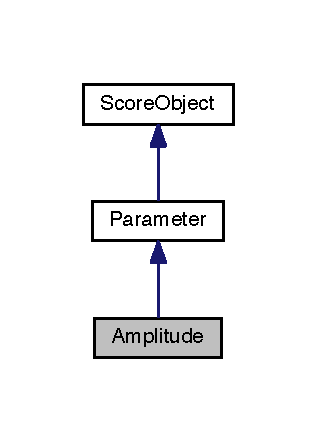
\includegraphics[width=152pt]{class_amplitude__inherit__graph}
\end{center}
\end{figure}


Collaboration diagram for Amplitude\-:\nopagebreak
\begin{figure}[H]
\begin{center}
\leavevmode
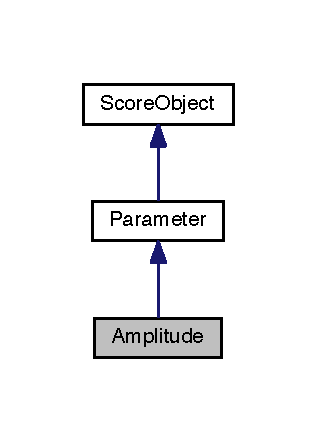
\includegraphics[width=152pt]{class_amplitude__coll__graph}
\end{center}
\end{figure}
\subsection*{Public Member Functions}
\begin{DoxyCompactItemize}
\item 
\hyperlink{class_amplitude_a41222cf45c46eb70625913595f95da50}{Amplitude} (\hyperlink{_score_core___score_object_8h_ab88aad89d974920ebfb0b0c9e46f61b4}{Args} as)
\item 
float \hyperlink{class_amplitude_a4d1360f1c95436bcef78b001c32ff7a6}{get\-Value\-Normalized} (void)
\item 
float \hyperlink{class_amplitude_a0dd0f3541b9d3a973a5d21b84cab0600}{get\-Value\-In\-Velocity} (void)
\end{DoxyCompactItemize}


\subsection{Constructor \& Destructor Documentation}
\hypertarget{class_amplitude_a41222cf45c46eb70625913595f95da50}{\index{Amplitude@{Amplitude}!Amplitude@{Amplitude}}
\index{Amplitude@{Amplitude}!Amplitude@{Amplitude}}
\subsubsection[{Amplitude}]{\setlength{\rightskip}{0pt plus 5cm}Amplitude\-::\-Amplitude (
\begin{DoxyParamCaption}
\item[{{\bf Args}}]{as}
\end{DoxyParamCaption}
)\hspace{0.3cm}{\ttfamily [inline]}}}\label{class_amplitude_a41222cf45c46eb70625913595f95da50}


\subsection{Member Function Documentation}
\hypertarget{class_amplitude_a0dd0f3541b9d3a973a5d21b84cab0600}{\index{Amplitude@{Amplitude}!get\-Value\-In\-Velocity@{get\-Value\-In\-Velocity}}
\index{get\-Value\-In\-Velocity@{get\-Value\-In\-Velocity}!Amplitude@{Amplitude}}
\subsubsection[{get\-Value\-In\-Velocity}]{\setlength{\rightskip}{0pt plus 5cm}float Amplitude\-::get\-Value\-In\-Velocity (
\begin{DoxyParamCaption}
\item[{void}]{}
\end{DoxyParamCaption}
)}}\label{class_amplitude_a0dd0f3541b9d3a973a5d21b84cab0600}
\hypertarget{class_amplitude_a4d1360f1c95436bcef78b001c32ff7a6}{\index{Amplitude@{Amplitude}!get\-Value\-Normalized@{get\-Value\-Normalized}}
\index{get\-Value\-Normalized@{get\-Value\-Normalized}!Amplitude@{Amplitude}}
\subsubsection[{get\-Value\-Normalized}]{\setlength{\rightskip}{0pt plus 5cm}float Amplitude\-::get\-Value\-Normalized (
\begin{DoxyParamCaption}
\item[{void}]{}
\end{DoxyParamCaption}
)}}\label{class_amplitude_a4d1360f1c95436bcef78b001c32ff7a6}


The documentation for this class was generated from the following file\-:\begin{DoxyCompactItemize}
\item 
Music\-Representation/\hyperlink{_score_core___parameter_8h}{Score\-Core\-\_\-\-Parameter.\-h}\end{DoxyCompactItemize}

\hypertarget{class_container}{\section{Container Class Reference}
\label{class_container}\index{Container@{Container}}
}


{\ttfamily \#include $<$Score\-Core\-\_\-\-Container.\-h$>$}



Inheritance diagram for Container\-:\nopagebreak
\begin{figure}[H]
\begin{center}
\leavevmode
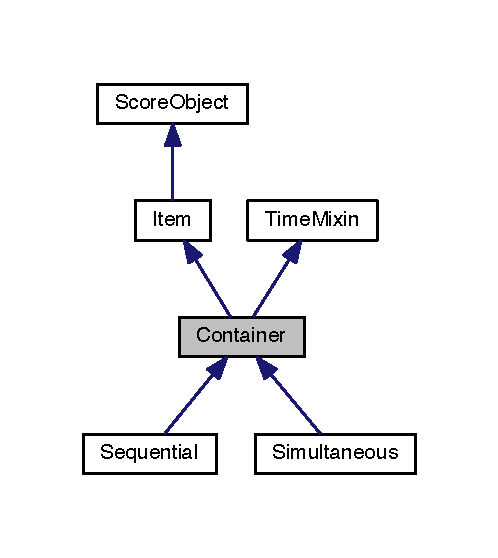
\includegraphics[width=239pt]{class_container__inherit__graph}
\end{center}
\end{figure}


Collaboration diagram for Container\-:\nopagebreak
\begin{figure}[H]
\begin{center}
\leavevmode
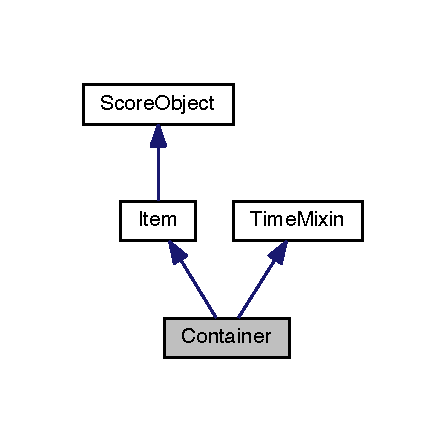
\includegraphics[width=214pt]{class_container__coll__graph}
\end{center}
\end{figure}
\subsection*{Public Member Functions}
\begin{DoxyCompactItemize}
\item 
\hyperlink{class_container_a58fe89314bc5e01d5f0a9b3b657c6b7d}{Container} (\hyperlink{_score_core___score_object_8h_ab88aad89d974920ebfb0b0c9e46f61b4}{Args} as)
\item 
std\-::vector$<$ \hyperlink{class_item}{Item} $>$ \hyperlink{class_container_a52e94ab27524bea68a6a9dd1646fa316}{get\-Items} (void)
\item 
void \hyperlink{class_container_a0de45ee721e564ecf487f2f042b9c554}{add\-Item} (\hyperlink{class_item}{Item} $\ast$)
\end{DoxyCompactItemize}


\subsection{Detailed Description}
\mbox{[}abstract class\mbox{]} A container contains one or more score items.

The variable items points to the items contained in a container. Because containers themself are items as well, a container can contain other containers to form a score hierarchy of containers and elements. However, a container must not contain itself. 

\subsection{Constructor \& Destructor Documentation}
\hypertarget{class_container_a58fe89314bc5e01d5f0a9b3b657c6b7d}{\index{Container@{Container}!Container@{Container}}
\index{Container@{Container}!Container@{Container}}
\subsubsection[{Container}]{\setlength{\rightskip}{0pt plus 5cm}Container\-::\-Container (
\begin{DoxyParamCaption}
\item[{{\bf Args}}]{as}
\end{DoxyParamCaption}
)}}\label{class_container_a58fe89314bc5e01d5f0a9b3b657c6b7d}
\hyperlink{class_container}{Container} constructor.

Arguments in Args as 
\begin{DoxyParams}{Parameters}
{\em vector$<$\-Item$>$} & items \\
\hline
{\em int} & offset\-Time \\
\hline
{\em int} & start\-Time \\
\hline
{\em int} & duration \\
\hline
{\em int} & end\-Time\\
\hline
\end{DoxyParams}
In addition all Args of constructors of \hyperlink{class_container}{Container} superclasses are supported.

T\-O\-D\-O\-: revise orig Strasheela doc\-: The optional argument 'items' expects a list of items which are contained in the container instance. (Additionally, items can be given by calling the method bilink\-Items.) A convenient shorthand notation for 'items' is the init method argument at record position 1. Example\-: init(My\-Items ...) 

\subsection{Member Function Documentation}
\hypertarget{class_container_a0de45ee721e564ecf487f2f042b9c554}{\index{Container@{Container}!add\-Item@{add\-Item}}
\index{add\-Item@{add\-Item}!Container@{Container}}
\subsubsection[{add\-Item}]{\setlength{\rightskip}{0pt plus 5cm}void Container\-::add\-Item (
\begin{DoxyParamCaption}
\item[{{\bf Item} $\ast$}]{}
\end{DoxyParamCaption}
)}}\label{class_container_a0de45ee721e564ecf487f2f042b9c554}
\hypertarget{class_container_a52e94ab27524bea68a6a9dd1646fa316}{\index{Container@{Container}!get\-Items@{get\-Items}}
\index{get\-Items@{get\-Items}!Container@{Container}}
\subsubsection[{get\-Items}]{\setlength{\rightskip}{0pt plus 5cm}std\-::vector$<${\bf Item}$>$ Container\-::get\-Items (
\begin{DoxyParamCaption}
\item[{void}]{}
\end{DoxyParamCaption}
)}}\label{class_container_a52e94ab27524bea68a6a9dd1646fa316}


The documentation for this class was generated from the following files\-:\begin{DoxyCompactItemize}
\item 
Music\-Representation/\hyperlink{_score_core___container_8h}{Score\-Core\-\_\-\-Container.\-h}\item 
Music\-Representation/\hyperlink{_score_core___container_8cpp}{Score\-Core\-\_\-\-Container.\-cpp}\end{DoxyCompactItemize}

\hypertarget{class_element}{\section{Element Class Reference}
\label{class_element}\index{Element@{Element}}
}


{\ttfamily \#include $<$Score\-Core\-\_\-\-Element.\-h$>$}



Inheritance diagram for Element\-:\nopagebreak
\begin{figure}[H]
\begin{center}
\leavevmode
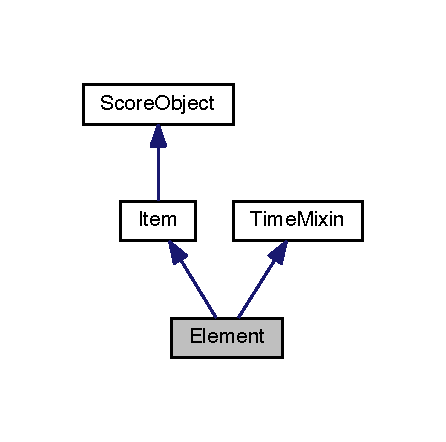
\includegraphics[width=214pt]{class_element__inherit__graph}
\end{center}
\end{figure}


Collaboration diagram for Element\-:\nopagebreak
\begin{figure}[H]
\begin{center}
\leavevmode
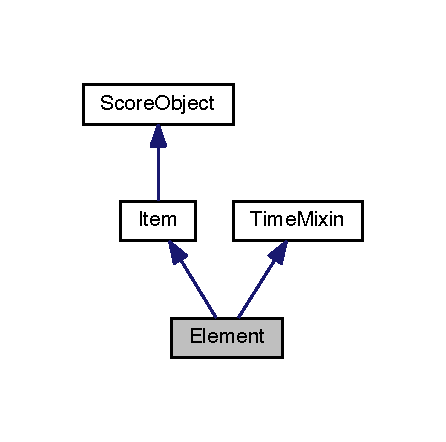
\includegraphics[width=214pt]{class_element__coll__graph}
\end{center}
\end{figure}
\subsection*{Public Member Functions}
\begin{DoxyCompactItemize}
\item 
\hyperlink{class_element_ad53dcf96e5ac05236ebb1a4b85987803}{Element} (\hyperlink{_score_core___score_object_8h_ab88aad89d974920ebfb0b0c9e46f61b4}{Args} as)
\end{DoxyCompactItemize}


\subsection{Constructor \& Destructor Documentation}
\hypertarget{class_element_ad53dcf96e5ac05236ebb1a4b85987803}{\index{Element@{Element}!Element@{Element}}
\index{Element@{Element}!Element@{Element}}
\subsubsection[{Element}]{\setlength{\rightskip}{0pt plus 5cm}Element\-::\-Element (
\begin{DoxyParamCaption}
\item[{{\bf Args}}]{as}
\end{DoxyParamCaption}
)}}\label{class_element_ad53dcf96e5ac05236ebb1a4b85987803}


The documentation for this class was generated from the following files\-:\begin{DoxyCompactItemize}
\item 
Music\-Representation/\hyperlink{_score_core___element_8h}{Score\-Core\-\_\-\-Element.\-h}\item 
Music\-Representation/\hyperlink{_score_core___element_8cpp}{Score\-Core\-\_\-\-Element.\-cpp}\end{DoxyCompactItemize}

\hypertarget{classget_arg}{\section{get\-Arg$<$ T $>$ Class Template Reference}
\label{classget_arg}\index{get\-Arg$<$ T $>$@{get\-Arg$<$ T $>$}}
}


{\ttfamily \#include $<$Score\-Core\-\_\-\-Type\-Args.\-h$>$}



Inheritance diagram for get\-Arg$<$ T $>$\-:\nopagebreak
\begin{figure}[H]
\begin{center}
\leavevmode
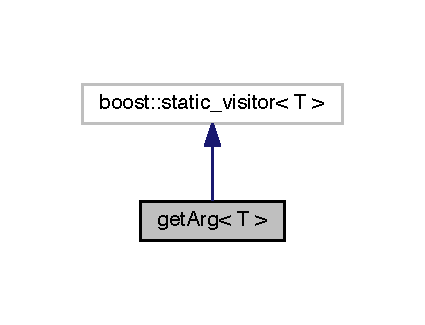
\includegraphics[width=204pt]{classget_arg__inherit__graph}
\end{center}
\end{figure}


Collaboration diagram for get\-Arg$<$ T $>$\-:\nopagebreak
\begin{figure}[H]
\begin{center}
\leavevmode
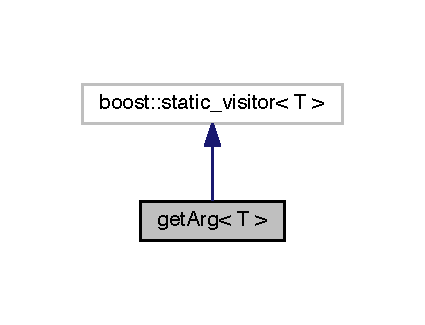
\includegraphics[width=204pt]{classget_arg__coll__graph}
\end{center}
\end{figure}
\subsection*{Public Member Functions}
\begin{DoxyCompactItemize}
\item 
T \hyperlink{classget_arg_a1cac113349006ef4fef741a43d826f94}{operator()} (const T \&t)
\item 
{\footnotesize template$<$typename U $>$ }\\T \hyperlink{classget_arg_a672364205c4d709a72596a285bcecae7}{operator()} (const U \&u)
\end{DoxyCompactItemize}


\subsection{Detailed Description}
\subsubsection*{template$<$typename T$>$class get\-Arg$<$ T $>$}

Defines compile-\/time checked accessors for (i.\-e. the values in the map type called Args). 

\subsection{Member Function Documentation}
\hypertarget{classget_arg_a1cac113349006ef4fef741a43d826f94}{\index{get\-Arg@{get\-Arg}!operator()@{operator()}}
\index{operator()@{operator()}!getArg@{get\-Arg}}
\subsubsection[{operator()}]{\setlength{\rightskip}{0pt plus 5cm}template$<$typename T $>$ T {\bf get\-Arg}$<$ T $>$\-::operator() (
\begin{DoxyParamCaption}
\item[{const T \&}]{t}
\end{DoxyParamCaption}
)\hspace{0.3cm}{\ttfamily [inline]}}}\label{classget_arg_a1cac113349006ef4fef741a43d826f94}
\hypertarget{classget_arg_a672364205c4d709a72596a285bcecae7}{\index{get\-Arg@{get\-Arg}!operator()@{operator()}}
\index{operator()@{operator()}!getArg@{get\-Arg}}
\subsubsection[{operator()}]{\setlength{\rightskip}{0pt plus 5cm}template$<$typename T $>$ template$<$typename U $>$ T {\bf get\-Arg}$<$ T $>$\-::operator() (
\begin{DoxyParamCaption}
\item[{const U \&}]{u}
\end{DoxyParamCaption}
)\hspace{0.3cm}{\ttfamily [inline]}}}\label{classget_arg_a672364205c4d709a72596a285bcecae7}


The documentation for this class was generated from the following file\-:\begin{DoxyCompactItemize}
\item 
Music\-Representation/\hyperlink{_score_core___type_args_8h}{Score\-Core\-\_\-\-Type\-Args.\-h}\end{DoxyCompactItemize}

\hypertarget{classget_int_arg}{\section{get\-Int\-Arg Class Reference}
\label{classget_int_arg}\index{get\-Int\-Arg@{get\-Int\-Arg}}
}


{\ttfamily \#include $<$Score\-Core\-\_\-\-Type\-Args.\-h$>$}



Inheritance diagram for get\-Int\-Arg\-:\nopagebreak
\begin{figure}[H]
\begin{center}
\leavevmode
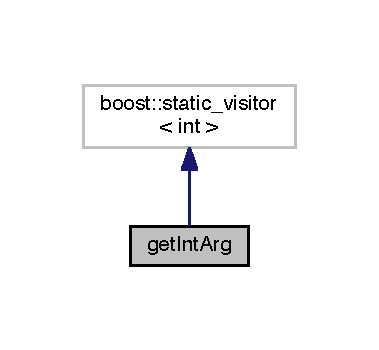
\includegraphics[width=182pt]{classget_int_arg__inherit__graph}
\end{center}
\end{figure}


Collaboration diagram for get\-Int\-Arg\-:\nopagebreak
\begin{figure}[H]
\begin{center}
\leavevmode
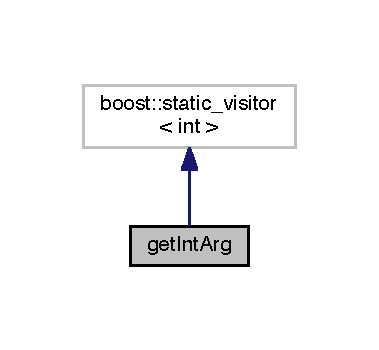
\includegraphics[width=182pt]{classget_int_arg__coll__graph}
\end{center}
\end{figure}
\subsection*{Public Member Functions}
\begin{DoxyCompactItemize}
\item 
int \hyperlink{classget_int_arg_a17317c109e19e8cb19a1cbb9686a39c3}{operator()} (std\-::string \&str) const 
\item 
int \hyperlink{classget_int_arg_ab9f67ca57c8172ee815014ce60b11798}{operator()} (int \&i) const 
\item 
int \hyperlink{classget_int_arg_ab24e7454d1a4e8de20041da5982c8683}{operator()} (\hyperlink{class_score_object}{Score\-Object} \&x) const 
\item 
int \hyperlink{classget_int_arg_a3735f850f683ad933beeeea562fafc8a}{operator()} (std\-::vector$<$ \hyperlink{class_score_object}{Score\-Object} $>$ \&xs) const 
\end{DoxyCompactItemize}


\subsection{Member Function Documentation}
\hypertarget{classget_int_arg_a17317c109e19e8cb19a1cbb9686a39c3}{\index{get\-Int\-Arg@{get\-Int\-Arg}!operator()@{operator()}}
\index{operator()@{operator()}!getIntArg@{get\-Int\-Arg}}
\subsubsection[{operator()}]{\setlength{\rightskip}{0pt plus 5cm}int get\-Int\-Arg\-::operator() (
\begin{DoxyParamCaption}
\item[{std\-::string \&}]{str}
\end{DoxyParamCaption}
) const}}\label{classget_int_arg_a17317c109e19e8cb19a1cbb9686a39c3}
\hypertarget{classget_int_arg_ab9f67ca57c8172ee815014ce60b11798}{\index{get\-Int\-Arg@{get\-Int\-Arg}!operator()@{operator()}}
\index{operator()@{operator()}!getIntArg@{get\-Int\-Arg}}
\subsubsection[{operator()}]{\setlength{\rightskip}{0pt plus 5cm}int get\-Int\-Arg\-::operator() (
\begin{DoxyParamCaption}
\item[{int \&}]{i}
\end{DoxyParamCaption}
) const}}\label{classget_int_arg_ab9f67ca57c8172ee815014ce60b11798}
\hypertarget{classget_int_arg_ab24e7454d1a4e8de20041da5982c8683}{\index{get\-Int\-Arg@{get\-Int\-Arg}!operator()@{operator()}}
\index{operator()@{operator()}!getIntArg@{get\-Int\-Arg}}
\subsubsection[{operator()}]{\setlength{\rightskip}{0pt plus 5cm}int get\-Int\-Arg\-::operator() (
\begin{DoxyParamCaption}
\item[{{\bf Score\-Object} \&}]{x}
\end{DoxyParamCaption}
) const}}\label{classget_int_arg_ab24e7454d1a4e8de20041da5982c8683}
\hypertarget{classget_int_arg_a3735f850f683ad933beeeea562fafc8a}{\index{get\-Int\-Arg@{get\-Int\-Arg}!operator()@{operator()}}
\index{operator()@{operator()}!getIntArg@{get\-Int\-Arg}}
\subsubsection[{operator()}]{\setlength{\rightskip}{0pt plus 5cm}int get\-Int\-Arg\-::operator() (
\begin{DoxyParamCaption}
\item[{std\-::vector$<$ {\bf Score\-Object} $>$ \&}]{xs}
\end{DoxyParamCaption}
) const}}\label{classget_int_arg_a3735f850f683ad933beeeea562fafc8a}


The documentation for this class was generated from the following files\-:\begin{DoxyCompactItemize}
\item 
Music\-Representation/\hyperlink{_score_core___type_args_8h}{Score\-Core\-\_\-\-Type\-Args.\-h}\item 
Music\-Representation/\hyperlink{_score_core___type_args_8cpp}{Score\-Core\-\_\-\-Type\-Args.\-cpp}\end{DoxyCompactItemize}

\hypertarget{classget_score_object_arg}{\section{get\-Score\-Object\-Arg Class Reference}
\label{classget_score_object_arg}\index{get\-Score\-Object\-Arg@{get\-Score\-Object\-Arg}}
}


{\ttfamily \#include $<$Score\-Core\-\_\-\-Type\-Args.\-h$>$}



Inheritance diagram for get\-Score\-Object\-Arg\-:\nopagebreak
\begin{figure}[H]
\begin{center}
\leavevmode
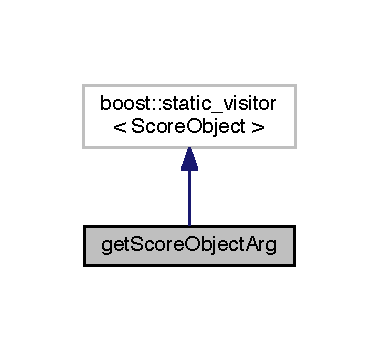
\includegraphics[width=182pt]{classget_score_object_arg__inherit__graph}
\end{center}
\end{figure}


Collaboration diagram for get\-Score\-Object\-Arg\-:\nopagebreak
\begin{figure}[H]
\begin{center}
\leavevmode
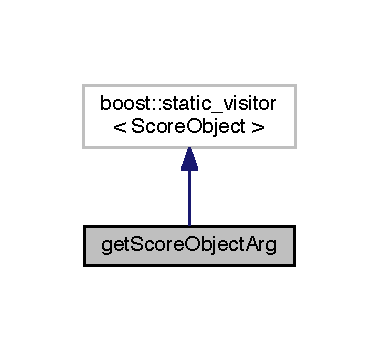
\includegraphics[width=182pt]{classget_score_object_arg__coll__graph}
\end{center}
\end{figure}
\subsection*{Public Member Functions}
\begin{DoxyCompactItemize}
\item 
\hyperlink{class_score_object}{Score\-Object} \hyperlink{classget_score_object_arg_a5c4ba390f0c95cf116441ea85564db54}{operator()} (std\-::string \&str) const 
\item 
\hyperlink{class_score_object}{Score\-Object} \hyperlink{classget_score_object_arg_a7127a547ad675123a0fa97d88abaf281}{operator()} (int \&i) const 
\item 
\hyperlink{class_score_object}{Score\-Object} \hyperlink{classget_score_object_arg_a11b4ad521c5e491b633be6a794afd5ec}{operator()} (\hyperlink{class_score_object}{Score\-Object} \&x) const 
\item 
\hyperlink{class_score_object}{Score\-Object} \hyperlink{classget_score_object_arg_aafd959b6293d33a3b6813da9658f63f3}{operator()} (std\-::vector$<$ \hyperlink{class_score_object}{Score\-Object} $>$ \&xs) const 
\end{DoxyCompactItemize}


\subsection{Member Function Documentation}
\hypertarget{classget_score_object_arg_a5c4ba390f0c95cf116441ea85564db54}{\index{get\-Score\-Object\-Arg@{get\-Score\-Object\-Arg}!operator()@{operator()}}
\index{operator()@{operator()}!getScoreObjectArg@{get\-Score\-Object\-Arg}}
\subsubsection[{operator()}]{\setlength{\rightskip}{0pt plus 5cm}{\bf Score\-Object} get\-Score\-Object\-Arg\-::operator() (
\begin{DoxyParamCaption}
\item[{std\-::string \&}]{str}
\end{DoxyParamCaption}
) const}}\label{classget_score_object_arg_a5c4ba390f0c95cf116441ea85564db54}
\hypertarget{classget_score_object_arg_a7127a547ad675123a0fa97d88abaf281}{\index{get\-Score\-Object\-Arg@{get\-Score\-Object\-Arg}!operator()@{operator()}}
\index{operator()@{operator()}!getScoreObjectArg@{get\-Score\-Object\-Arg}}
\subsubsection[{operator()}]{\setlength{\rightskip}{0pt plus 5cm}{\bf Score\-Object} get\-Score\-Object\-Arg\-::operator() (
\begin{DoxyParamCaption}
\item[{int \&}]{i}
\end{DoxyParamCaption}
) const}}\label{classget_score_object_arg_a7127a547ad675123a0fa97d88abaf281}
\hypertarget{classget_score_object_arg_a11b4ad521c5e491b633be6a794afd5ec}{\index{get\-Score\-Object\-Arg@{get\-Score\-Object\-Arg}!operator()@{operator()}}
\index{operator()@{operator()}!getScoreObjectArg@{get\-Score\-Object\-Arg}}
\subsubsection[{operator()}]{\setlength{\rightskip}{0pt plus 5cm}{\bf Score\-Object} get\-Score\-Object\-Arg\-::operator() (
\begin{DoxyParamCaption}
\item[{{\bf Score\-Object} \&}]{x}
\end{DoxyParamCaption}
) const}}\label{classget_score_object_arg_a11b4ad521c5e491b633be6a794afd5ec}
\hypertarget{classget_score_object_arg_aafd959b6293d33a3b6813da9658f63f3}{\index{get\-Score\-Object\-Arg@{get\-Score\-Object\-Arg}!operator()@{operator()}}
\index{operator()@{operator()}!getScoreObjectArg@{get\-Score\-Object\-Arg}}
\subsubsection[{operator()}]{\setlength{\rightskip}{0pt plus 5cm}{\bf Score\-Object} get\-Score\-Object\-Arg\-::operator() (
\begin{DoxyParamCaption}
\item[{std\-::vector$<$ {\bf Score\-Object} $>$ \&}]{xs}
\end{DoxyParamCaption}
) const}}\label{classget_score_object_arg_aafd959b6293d33a3b6813da9658f63f3}


The documentation for this class was generated from the following files\-:\begin{DoxyCompactItemize}
\item 
Music\-Representation/\hyperlink{_score_core___type_args_8h}{Score\-Core\-\_\-\-Type\-Args.\-h}\item 
Music\-Representation/\hyperlink{_score_core___type_args_8cpp}{Score\-Core\-\_\-\-Type\-Args.\-cpp}\end{DoxyCompactItemize}

\hypertarget{classget_string_arg}{\section{get\-String\-Arg Class Reference}
\label{classget_string_arg}\index{get\-String\-Arg@{get\-String\-Arg}}
}


{\ttfamily \#include $<$Score\-Core\-\_\-\-Type\-Args.\-h$>$}



Inheritance diagram for get\-String\-Arg\-:\nopagebreak
\begin{figure}[H]
\begin{center}
\leavevmode
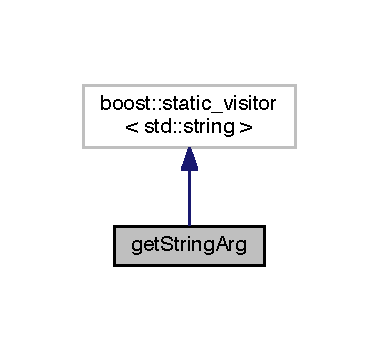
\includegraphics[width=182pt]{classget_string_arg__inherit__graph}
\end{center}
\end{figure}


Collaboration diagram for get\-String\-Arg\-:\nopagebreak
\begin{figure}[H]
\begin{center}
\leavevmode
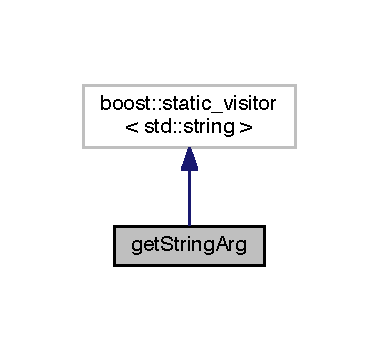
\includegraphics[width=182pt]{classget_string_arg__coll__graph}
\end{center}
\end{figure}
\subsection*{Public Member Functions}
\begin{DoxyCompactItemize}
\item 
std\-::string \hyperlink{classget_string_arg_a0a467143ebba5978fe9a363d0d31ff3b}{operator()} (std\-::string \&str) const 
\item 
std\-::string \hyperlink{classget_string_arg_adae14b089252bc8e2203da2a3c74712d}{operator()} (int \&i) const 
\item 
std\-::string \hyperlink{classget_string_arg_a9e7d8e2a11b813c4a4dc3d7bbc610d82}{operator()} (\hyperlink{class_score_object}{Score\-Object} \&x) const 
\item 
std\-::string \hyperlink{classget_string_arg_ab910bbfbe751febe0e984e12a903bf58}{operator()} (std\-::vector$<$ \hyperlink{class_score_object}{Score\-Object} $>$ \&xs) const 
\end{DoxyCompactItemize}


\subsection{Detailed Description}
Defines compile-\/time checked accessors for every type given to Args (i.\-e. the values in the map type called Args). 

\subsection{Member Function Documentation}
\hypertarget{classget_string_arg_a0a467143ebba5978fe9a363d0d31ff3b}{\index{get\-String\-Arg@{get\-String\-Arg}!operator()@{operator()}}
\index{operator()@{operator()}!getStringArg@{get\-String\-Arg}}
\subsubsection[{operator()}]{\setlength{\rightskip}{0pt plus 5cm}std\-::string get\-String\-Arg\-::operator() (
\begin{DoxyParamCaption}
\item[{std\-::string \&}]{str}
\end{DoxyParamCaption}
) const}}\label{classget_string_arg_a0a467143ebba5978fe9a363d0d31ff3b}
\hypertarget{classget_string_arg_adae14b089252bc8e2203da2a3c74712d}{\index{get\-String\-Arg@{get\-String\-Arg}!operator()@{operator()}}
\index{operator()@{operator()}!getStringArg@{get\-String\-Arg}}
\subsubsection[{operator()}]{\setlength{\rightskip}{0pt plus 5cm}string get\-String\-Arg\-::operator() (
\begin{DoxyParamCaption}
\item[{int \&}]{i}
\end{DoxyParamCaption}
) const}}\label{classget_string_arg_adae14b089252bc8e2203da2a3c74712d}
\hypertarget{classget_string_arg_a9e7d8e2a11b813c4a4dc3d7bbc610d82}{\index{get\-String\-Arg@{get\-String\-Arg}!operator()@{operator()}}
\index{operator()@{operator()}!getStringArg@{get\-String\-Arg}}
\subsubsection[{operator()}]{\setlength{\rightskip}{0pt plus 5cm}string get\-String\-Arg\-::operator() (
\begin{DoxyParamCaption}
\item[{{\bf Score\-Object} \&}]{x}
\end{DoxyParamCaption}
) const}}\label{classget_string_arg_a9e7d8e2a11b813c4a4dc3d7bbc610d82}
\hypertarget{classget_string_arg_ab910bbfbe751febe0e984e12a903bf58}{\index{get\-String\-Arg@{get\-String\-Arg}!operator()@{operator()}}
\index{operator()@{operator()}!getStringArg@{get\-String\-Arg}}
\subsubsection[{operator()}]{\setlength{\rightskip}{0pt plus 5cm}string get\-String\-Arg\-::operator() (
\begin{DoxyParamCaption}
\item[{std\-::vector$<$ {\bf Score\-Object} $>$ \&}]{xs}
\end{DoxyParamCaption}
) const}}\label{classget_string_arg_ab910bbfbe751febe0e984e12a903bf58}


The documentation for this class was generated from the following files\-:\begin{DoxyCompactItemize}
\item 
Music\-Representation/\hyperlink{_score_core___type_args_8h}{Score\-Core\-\_\-\-Type\-Args.\-h}\item 
Music\-Representation/\hyperlink{_score_core___type_args_8cpp}{Score\-Core\-\_\-\-Type\-Args.\-cpp}\end{DoxyCompactItemize}

\hypertarget{classget_vector_of_score_objects_arg}{\section{get\-Vector\-Of\-Score\-Objects\-Arg Class Reference}
\label{classget_vector_of_score_objects_arg}\index{get\-Vector\-Of\-Score\-Objects\-Arg@{get\-Vector\-Of\-Score\-Objects\-Arg}}
}


{\ttfamily \#include $<$Score\-Core\-\_\-\-Type\-Args.\-h$>$}



Inheritance diagram for get\-Vector\-Of\-Score\-Objects\-Arg\-:\nopagebreak
\begin{figure}[H]
\begin{center}
\leavevmode
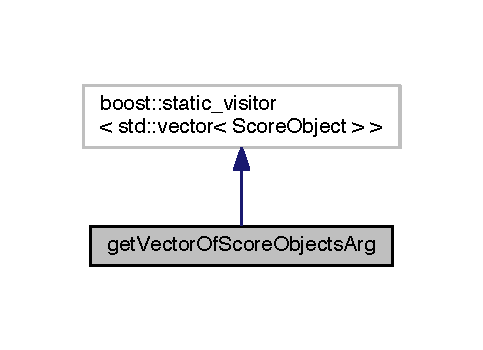
\includegraphics[width=232pt]{classget_vector_of_score_objects_arg__inherit__graph}
\end{center}
\end{figure}


Collaboration diagram for get\-Vector\-Of\-Score\-Objects\-Arg\-:\nopagebreak
\begin{figure}[H]
\begin{center}
\leavevmode
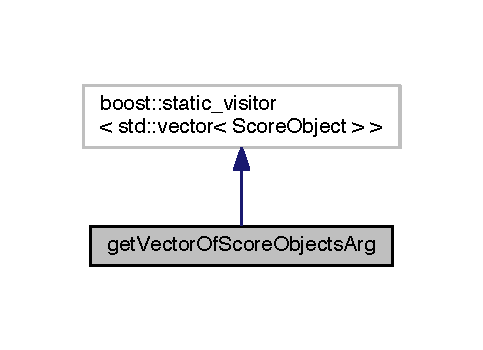
\includegraphics[width=232pt]{classget_vector_of_score_objects_arg__coll__graph}
\end{center}
\end{figure}
\subsection*{Public Member Functions}
\begin{DoxyCompactItemize}
\item 
std\-::vector$<$ \hyperlink{class_score_object}{Score\-Object} $>$ \hyperlink{classget_vector_of_score_objects_arg_a7426c57dfb3402f2e9054c9ac85c0647}{operator()} (std\-::string \&str) const 
\item 
std\-::vector$<$ \hyperlink{class_score_object}{Score\-Object} $>$ \hyperlink{classget_vector_of_score_objects_arg_a222f7c2c38e8ba39faa299fb90d273dc}{operator()} (int \&i) const 
\item 
std\-::vector$<$ \hyperlink{class_score_object}{Score\-Object} $>$ \hyperlink{classget_vector_of_score_objects_arg_a1cea57cf980328cd3d8e36ca0ce953ba}{operator()} (\hyperlink{class_score_object}{Score\-Object} \&x) const 
\item 
std\-::vector$<$ \hyperlink{class_score_object}{Score\-Object} $>$ \hyperlink{classget_vector_of_score_objects_arg_acb057628f3de707e20414112135d2504}{operator()} (std\-::vector$<$ \hyperlink{class_score_object}{Score\-Object} $>$ \&xs) const 
\end{DoxyCompactItemize}


\subsection{Member Function Documentation}
\hypertarget{classget_vector_of_score_objects_arg_a7426c57dfb3402f2e9054c9ac85c0647}{\index{get\-Vector\-Of\-Score\-Objects\-Arg@{get\-Vector\-Of\-Score\-Objects\-Arg}!operator()@{operator()}}
\index{operator()@{operator()}!getVectorOfScoreObjectsArg@{get\-Vector\-Of\-Score\-Objects\-Arg}}
\subsubsection[{operator()}]{\setlength{\rightskip}{0pt plus 5cm}std\-::vector$<${\bf Score\-Object}$>$ get\-Vector\-Of\-Score\-Objects\-Arg\-::operator() (
\begin{DoxyParamCaption}
\item[{std\-::string \&}]{str}
\end{DoxyParamCaption}
) const}}\label{classget_vector_of_score_objects_arg_a7426c57dfb3402f2e9054c9ac85c0647}
\hypertarget{classget_vector_of_score_objects_arg_a222f7c2c38e8ba39faa299fb90d273dc}{\index{get\-Vector\-Of\-Score\-Objects\-Arg@{get\-Vector\-Of\-Score\-Objects\-Arg}!operator()@{operator()}}
\index{operator()@{operator()}!getVectorOfScoreObjectsArg@{get\-Vector\-Of\-Score\-Objects\-Arg}}
\subsubsection[{operator()}]{\setlength{\rightskip}{0pt plus 5cm}std\-::vector$<$ {\bf Score\-Object} $>$ get\-Vector\-Of\-Score\-Objects\-Arg\-::operator() (
\begin{DoxyParamCaption}
\item[{int \&}]{i}
\end{DoxyParamCaption}
) const}}\label{classget_vector_of_score_objects_arg_a222f7c2c38e8ba39faa299fb90d273dc}
\hypertarget{classget_vector_of_score_objects_arg_a1cea57cf980328cd3d8e36ca0ce953ba}{\index{get\-Vector\-Of\-Score\-Objects\-Arg@{get\-Vector\-Of\-Score\-Objects\-Arg}!operator()@{operator()}}
\index{operator()@{operator()}!getVectorOfScoreObjectsArg@{get\-Vector\-Of\-Score\-Objects\-Arg}}
\subsubsection[{operator()}]{\setlength{\rightskip}{0pt plus 5cm}std\-::vector$<$ {\bf Score\-Object} $>$ get\-Vector\-Of\-Score\-Objects\-Arg\-::operator() (
\begin{DoxyParamCaption}
\item[{{\bf Score\-Object} \&}]{x}
\end{DoxyParamCaption}
) const}}\label{classget_vector_of_score_objects_arg_a1cea57cf980328cd3d8e36ca0ce953ba}
\hypertarget{classget_vector_of_score_objects_arg_acb057628f3de707e20414112135d2504}{\index{get\-Vector\-Of\-Score\-Objects\-Arg@{get\-Vector\-Of\-Score\-Objects\-Arg}!operator()@{operator()}}
\index{operator()@{operator()}!getVectorOfScoreObjectsArg@{get\-Vector\-Of\-Score\-Objects\-Arg}}
\subsubsection[{operator()}]{\setlength{\rightskip}{0pt plus 5cm}std\-::vector$<$ {\bf Score\-Object} $>$ get\-Vector\-Of\-Score\-Objects\-Arg\-::operator() (
\begin{DoxyParamCaption}
\item[{std\-::vector$<$ {\bf Score\-Object} $>$ \&}]{xs}
\end{DoxyParamCaption}
) const}}\label{classget_vector_of_score_objects_arg_acb057628f3de707e20414112135d2504}


The documentation for this class was generated from the following files\-:\begin{DoxyCompactItemize}
\item 
Music\-Representation/\hyperlink{_score_core___type_args_8h}{Score\-Core\-\_\-\-Type\-Args.\-h}\item 
Music\-Representation/\hyperlink{_score_core___type_args_8cpp}{Score\-Core\-\_\-\-Type\-Args.\-cpp}\end{DoxyCompactItemize}

\hypertarget{class_item}{\section{Item Class Reference}
\label{class_item}\index{Item@{Item}}
}


{\ttfamily \#include $<$Score\-Core\-\_\-\-Item.\-h$>$}



Inheritance diagram for Item\-:\nopagebreak
\begin{figure}[H]
\begin{center}
\leavevmode
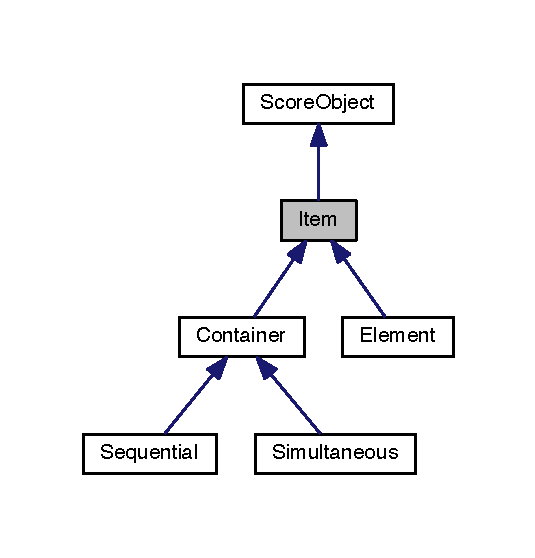
\includegraphics[width=257pt]{class_item__inherit__graph}
\end{center}
\end{figure}


Collaboration diagram for Item\-:\nopagebreak
\begin{figure}[H]
\begin{center}
\leavevmode
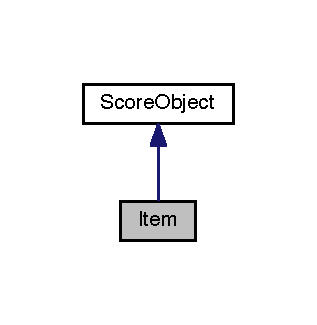
\includegraphics[width=152pt]{class_item__coll__graph}
\end{center}
\end{figure}
\subsection*{Public Member Functions}
\begin{DoxyCompactItemize}
\item 
\hyperlink{class_item_aaa8fbe0a8f0efb5f152d81cf260a6411}{Item} (\hyperlink{_score_core___score_object_8h_ab88aad89d974920ebfb0b0c9e46f61b4}{Args} as)
\item 
std\-::vector$<$ \hyperlink{class_parameter}{Parameter} $\ast$ $>$ \hyperlink{class_item_a087719491ab662eff4d0cd9c4a50a2ae}{get\-Parameters} (void)
\item 
\hyperlink{class_container}{Container} $\ast$ \hyperlink{class_item_a0d8d2ccd1a81ecb76fdf938fa6bf0d15}{get\-Container} (void)
\item 
void \hyperlink{class_item_af519b6c40476ed375fe36db754ae709e}{bilink\-Parameters} (std\-::vector$<$ \hyperlink{class_parameter}{Parameter} $\ast$ $>$ ps)
\end{DoxyCompactItemize}


\subsection{Constructor \& Destructor Documentation}
\hypertarget{class_item_aaa8fbe0a8f0efb5f152d81cf260a6411}{\index{Item@{Item}!Item@{Item}}
\index{Item@{Item}!Item@{Item}}
\subsubsection[{Item}]{\setlength{\rightskip}{0pt plus 5cm}Item\-::\-Item (
\begin{DoxyParamCaption}
\item[{{\bf Args}}]{as}
\end{DoxyParamCaption}
)}}\label{class_item_aaa8fbe0a8f0efb5f152d81cf260a6411}


\subsection{Member Function Documentation}
\hypertarget{class_item_af519b6c40476ed375fe36db754ae709e}{\index{Item@{Item}!bilink\-Parameters@{bilink\-Parameters}}
\index{bilink\-Parameters@{bilink\-Parameters}!Item@{Item}}
\subsubsection[{bilink\-Parameters}]{\setlength{\rightskip}{0pt plus 5cm}void Item\-::bilink\-Parameters (
\begin{DoxyParamCaption}
\item[{std\-::vector$<$ {\bf Parameter} $\ast$ $>$}]{ps}
\end{DoxyParamCaption}
)}}\label{class_item_af519b6c40476ed375fe36db754ae709e}
\mbox{[}aux method\mbox{]} Parameters and \hyperlink{class_item}{Item} $\ast$this are bidirectional linked. Method must not be called by user (only by designer of class with additional parameters). \hypertarget{class_item_a0d8d2ccd1a81ecb76fdf938fa6bf0d15}{\index{Item@{Item}!get\-Container@{get\-Container}}
\index{get\-Container@{get\-Container}!Item@{Item}}
\subsubsection[{get\-Container}]{\setlength{\rightskip}{0pt plus 5cm}{\bf Container} $\ast$ Item\-::get\-Container (
\begin{DoxyParamCaption}
\item[{void}]{}
\end{DoxyParamCaption}
)}}\label{class_item_a0d8d2ccd1a81ecb76fdf938fa6bf0d15}
\hypertarget{class_item_a087719491ab662eff4d0cd9c4a50a2ae}{\index{Item@{Item}!get\-Parameters@{get\-Parameters}}
\index{get\-Parameters@{get\-Parameters}!Item@{Item}}
\subsubsection[{get\-Parameters}]{\setlength{\rightskip}{0pt plus 5cm}std\-::vector$<$ {\bf Parameter} $\ast$ $>$ Item\-::get\-Parameters (
\begin{DoxyParamCaption}
\item[{void}]{}
\end{DoxyParamCaption}
)}}\label{class_item_a087719491ab662eff4d0cd9c4a50a2ae}


The documentation for this class was generated from the following files\-:\begin{DoxyCompactItemize}
\item 
Music\-Representation/\hyperlink{_score_core___item_8h}{Score\-Core\-\_\-\-Item.\-h}\item 
Music\-Representation/\hyperlink{_score_core___item_8cpp}{Score\-Core\-\_\-\-Item.\-cpp}\end{DoxyCompactItemize}

\hypertarget{class_parameter}{\section{Parameter Class Reference}
\label{class_parameter}\index{Parameter@{Parameter}}
}


{\ttfamily \#include $<$Score\-Core\-\_\-\-Parameter.\-h$>$}



Inheritance diagram for Parameter\-:\nopagebreak
\begin{figure}[H]
\begin{center}
\leavevmode
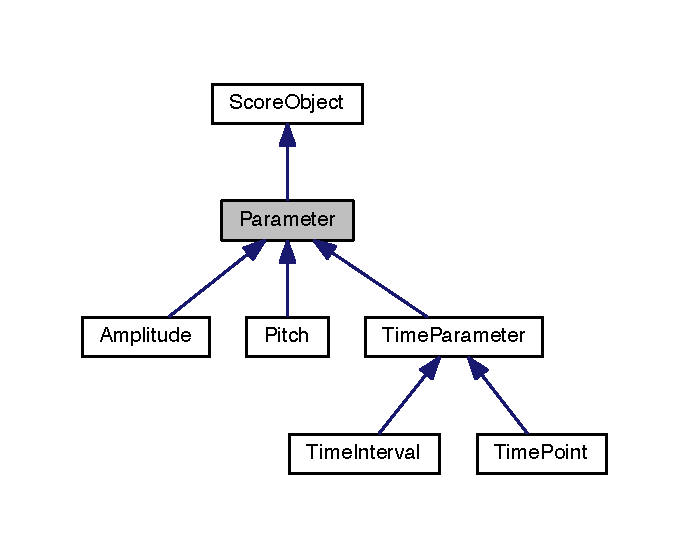
\includegraphics[width=331pt]{class_parameter__inherit__graph}
\end{center}
\end{figure}


Collaboration diagram for Parameter\-:\nopagebreak
\begin{figure}[H]
\begin{center}
\leavevmode
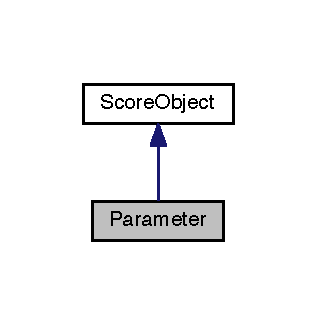
\includegraphics[width=152pt]{class_parameter__coll__graph}
\end{center}
\end{figure}
\subsection*{Public Member Functions}
\begin{DoxyCompactItemize}
\item 
\hyperlink{class_parameter_a254b32e69ff3548d6e7fd04347fdd5cf}{Parameter} (\hyperlink{_score_core___score_object_8h_ab88aad89d974920ebfb0b0c9e46f61b4}{Args} as)
\item 
int \hyperlink{class_parameter_a4459b636c3993ba40664ce8a53dad2c1}{get\-Value} (void)
\item 
std\-::string \hyperlink{class_parameter_a0688af42890903c327ccf0b2373bff34}{get\-Unit} (void)
\item 
\hyperlink{class_item}{Item} $\ast$ \hyperlink{class_parameter_ac2009f29ab47b8b68ae8739b348ec2c2}{get\-Item} (void)
\item 
void \hyperlink{class_parameter_ae7ac31fdbb6079bd96b3ab1034d127e0}{set\-Item} (\hyperlink{class_item}{Item} $\ast$)
\end{DoxyCompactItemize}


\subsection{Detailed Description}
\mbox{[}semi abstract class\mbox{]} Musical parameters are the basic magnitudes in a music representation; examples are the parameters duration, amplitude and pitch, which add information to a note. A parameter is represented by an own class (i.\-e. not just as a instance variables of score items, as in most other composition environments) to allow the expression of additional information on the parameter besides the actual parameter value. For instance, a single numeric value for a pitch is ambitious, it could express a frequency, a M\-I\-D\-I-\/keynumber, M\-I\-D\-I-\/cents, a scale degree etc. Therefore, a parameter allows to specify the unit of measurement explicitly. The unit is mainly used when exporting the score. Also, due to bidirectional links between nested score objects, all information stored in a score can be accessed from a parameter object (using member function get\-Item). Users should ensure that parameters have corresponding units when constraining the relation between multiple parameters. For efficiency, the parameter value is limited to integer values and integer variable (planned\-: float variables). However, due to the flexibility of the unit, these values can be mapped to arbitrary other data (e.\-g. midicent integer to frequency float). 

\subsection{Constructor \& Destructor Documentation}
\hypertarget{class_parameter_a254b32e69ff3548d6e7fd04347fdd5cf}{\index{Parameter@{Parameter}!Parameter@{Parameter}}
\index{Parameter@{Parameter}!Parameter@{Parameter}}
\subsubsection[{Parameter}]{\setlength{\rightskip}{0pt plus 5cm}Parameter\-::\-Parameter (
\begin{DoxyParamCaption}
\item[{{\bf Args}}]{as}
\end{DoxyParamCaption}
)}}\label{class_parameter_a254b32e69ff3548d6e7fd04347fdd5cf}
Args\-: int value\-: the parameter value string unit\-: parameter unit of measurement

and Args of \hyperlink{class_score_object}{Score\-Object} 

\subsection{Member Function Documentation}
\hypertarget{class_parameter_ac2009f29ab47b8b68ae8739b348ec2c2}{\index{Parameter@{Parameter}!get\-Item@{get\-Item}}
\index{get\-Item@{get\-Item}!Parameter@{Parameter}}
\subsubsection[{get\-Item}]{\setlength{\rightskip}{0pt plus 5cm}{\bf Item}$\ast$ Parameter\-::get\-Item (
\begin{DoxyParamCaption}
\item[{void}]{}
\end{DoxyParamCaption}
)}}\label{class_parameter_ac2009f29ab47b8b68ae8739b348ec2c2}
\hypertarget{class_parameter_a0688af42890903c327ccf0b2373bff34}{\index{Parameter@{Parameter}!get\-Unit@{get\-Unit}}
\index{get\-Unit@{get\-Unit}!Parameter@{Parameter}}
\subsubsection[{get\-Unit}]{\setlength{\rightskip}{0pt plus 5cm}std\-::string Parameter\-::get\-Unit (
\begin{DoxyParamCaption}
\item[{void}]{}
\end{DoxyParamCaption}
)}}\label{class_parameter_a0688af42890903c327ccf0b2373bff34}
\hypertarget{class_parameter_a4459b636c3993ba40664ce8a53dad2c1}{\index{Parameter@{Parameter}!get\-Value@{get\-Value}}
\index{get\-Value@{get\-Value}!Parameter@{Parameter}}
\subsubsection[{get\-Value}]{\setlength{\rightskip}{0pt plus 5cm}int Parameter\-::get\-Value (
\begin{DoxyParamCaption}
\item[{void}]{}
\end{DoxyParamCaption}
)}}\label{class_parameter_a4459b636c3993ba40664ce8a53dad2c1}
\hypertarget{class_parameter_ae7ac31fdbb6079bd96b3ab1034d127e0}{\index{Parameter@{Parameter}!set\-Item@{set\-Item}}
\index{set\-Item@{set\-Item}!Parameter@{Parameter}}
\subsubsection[{set\-Item}]{\setlength{\rightskip}{0pt plus 5cm}void Parameter\-::set\-Item (
\begin{DoxyParamCaption}
\item[{{\bf Item} $\ast$}]{i}
\end{DoxyParamCaption}
)}}\label{class_parameter_ae7ac31fdbb6079bd96b3ab1034d127e0}
\%\% \mbox{[}aux method\mbox{]} Method must not be called by user (must only used by \hyperlink{class_item_af519b6c40476ed375fe36db754ae709e}{Item\-::bilink\-Parameters}). \% 

The documentation for this class was generated from the following files\-:\begin{DoxyCompactItemize}
\item 
Music\-Representation/\hyperlink{_score_core___parameter_8h}{Score\-Core\-\_\-\-Parameter.\-h}\item 
Music\-Representation/\hyperlink{_score_core___parameter_8cpp}{Score\-Core\-\_\-\-Parameter.\-cpp}\end{DoxyCompactItemize}

\hypertarget{class_pitch}{\section{Pitch Class Reference}
\label{class_pitch}\index{Pitch@{Pitch}}
}


{\ttfamily \#include $<$Score\-Core\-\_\-\-Parameter.\-h$>$}



Inheritance diagram for Pitch\-:\nopagebreak
\begin{figure}[H]
\begin{center}
\leavevmode
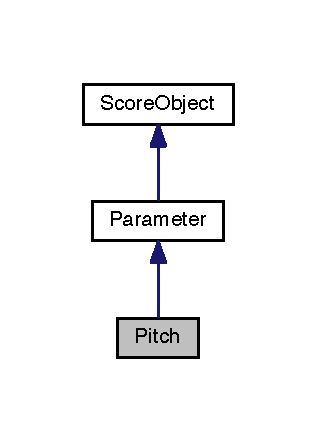
\includegraphics[width=152pt]{class_pitch__inherit__graph}
\end{center}
\end{figure}


Collaboration diagram for Pitch\-:\nopagebreak
\begin{figure}[H]
\begin{center}
\leavevmode
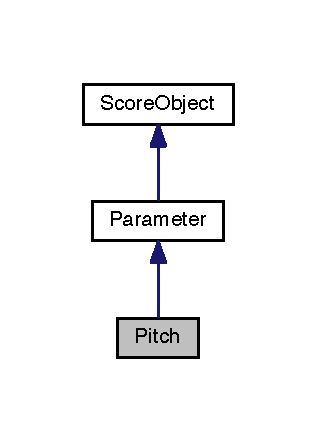
\includegraphics[width=152pt]{class_pitch__coll__graph}
\end{center}
\end{figure}
\subsection*{Public Member Functions}
\begin{DoxyCompactItemize}
\item 
\hyperlink{class_pitch_a6a92270f79cd0b7e67d5fe62b0b8acf9}{Pitch} (\hyperlink{_score_core___score_object_8h_ab88aad89d974920ebfb0b0c9e46f61b4}{Args} as)
\item 
float \hyperlink{class_pitch_a8c9dff38c999241c9420d5346c174b4b}{get\-Value\-In\-Midi} (void)
\item 
float \hyperlink{class_pitch_ab7a3da9aa96e8cc446d326ca43e49a38}{get\-Value\-In\-Midi} (std\-::map$<$ std\-::string, int $>$ tuning\-Table)
\end{DoxyCompactItemize}


\subsection{Constructor \& Destructor Documentation}
\hypertarget{class_pitch_a6a92270f79cd0b7e67d5fe62b0b8acf9}{\index{Pitch@{Pitch}!Pitch@{Pitch}}
\index{Pitch@{Pitch}!Pitch@{Pitch}}
\subsubsection[{Pitch}]{\setlength{\rightskip}{0pt plus 5cm}Pitch\-::\-Pitch (
\begin{DoxyParamCaption}
\item[{{\bf Args}}]{as}
\end{DoxyParamCaption}
)\hspace{0.3cm}{\ttfamily [inline]}}}\label{class_pitch_a6a92270f79cd0b7e67d5fe62b0b8acf9}


\subsection{Member Function Documentation}
\hypertarget{class_pitch_a8c9dff38c999241c9420d5346c174b4b}{\index{Pitch@{Pitch}!get\-Value\-In\-Midi@{get\-Value\-In\-Midi}}
\index{get\-Value\-In\-Midi@{get\-Value\-In\-Midi}!Pitch@{Pitch}}
\subsubsection[{get\-Value\-In\-Midi}]{\setlength{\rightskip}{0pt plus 5cm}float Pitch\-::get\-Value\-In\-Midi (
\begin{DoxyParamCaption}
\item[{void}]{}
\end{DoxyParamCaption}
)}}\label{class_pitch_a8c9dff38c999241c9420d5346c174b4b}
\hypertarget{class_pitch_ab7a3da9aa96e8cc446d326ca43e49a38}{\index{Pitch@{Pitch}!get\-Value\-In\-Midi@{get\-Value\-In\-Midi}}
\index{get\-Value\-In\-Midi@{get\-Value\-In\-Midi}!Pitch@{Pitch}}
\subsubsection[{get\-Value\-In\-Midi}]{\setlength{\rightskip}{0pt plus 5cm}float Pitch\-::get\-Value\-In\-Midi (
\begin{DoxyParamCaption}
\item[{std\-::map$<$ std\-::string, int $>$}]{tuning\-Table}
\end{DoxyParamCaption}
)}}\label{class_pitch_ab7a3da9aa96e8cc446d326ca43e49a38}


The documentation for this class was generated from the following file\-:\begin{DoxyCompactItemize}
\item 
Music\-Representation/\hyperlink{_score_core___parameter_8h}{Score\-Core\-\_\-\-Parameter.\-h}\end{DoxyCompactItemize}

\hypertarget{class_score_object}{\section{Score\-Object Class Reference}
\label{class_score_object}\index{Score\-Object@{Score\-Object}}
}


{\ttfamily \#include $<$Score\-Core\-\_\-\-Score\-Object.\-h$>$}



Inheritance diagram for Score\-Object\-:\nopagebreak
\begin{figure}[H]
\begin{center}
\leavevmode
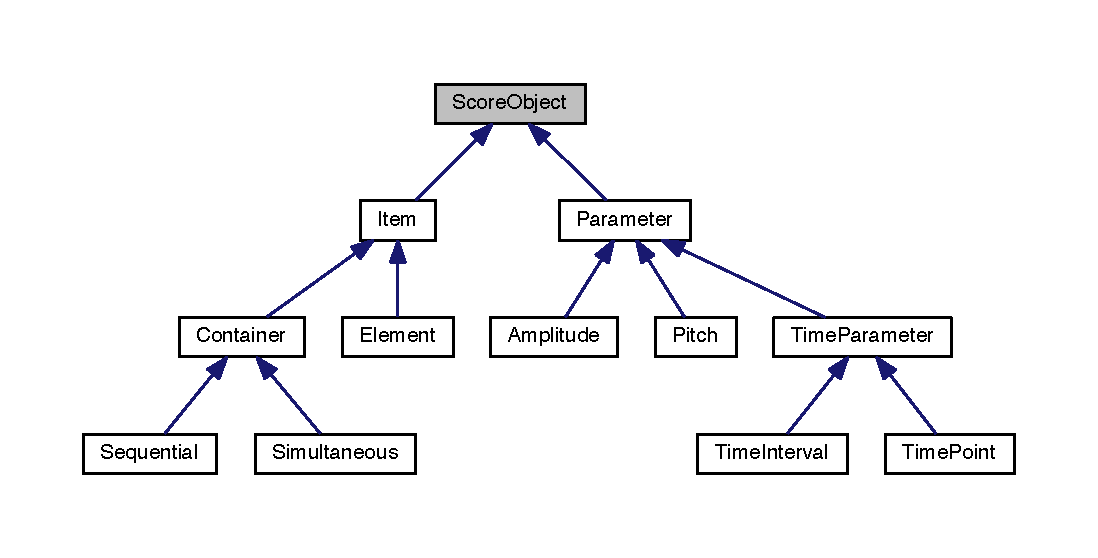
\includegraphics[width=350pt]{class_score_object__inherit__graph}
\end{center}
\end{figure}
\subsection*{Public Member Functions}
\begin{DoxyCompactItemize}
\item 
\hyperlink{class_score_object_a5d48b3ff7db868ad8d18716971d2e7c0}{Score\-Object} (\hyperlink{_score_core___score_object_8h_ab88aad89d974920ebfb0b0c9e46f61b4}{Args} as)
\item 
std\-::vector$<$ std\-::string $>$ \hyperlink{class_score_object_a10003206c88edf43e25180ddd06b8ad9}{get\-Info} (void)
\item 
void \hyperlink{class_score_object_a89b5be30134e8d77dbe1c253bc009b08}{add\-Info} (std\-::string my\-Info)
\item 
bool \hyperlink{class_score_object_a2625bd41018f22bcb9a64e2664cb9908}{has\-This\-Info} (std\-::string my\-Info)
\end{DoxyCompactItemize}


\subsection{Detailed Description}
\mbox{[}abstract class\mbox{]} The most general data type for score data is a \hyperlink{class_score_object}{Score\-Object}. 

\subsection{Constructor \& Destructor Documentation}
\hypertarget{class_score_object_a5d48b3ff7db868ad8d18716971d2e7c0}{\index{Score\-Object@{Score\-Object}!Score\-Object@{Score\-Object}}
\index{Score\-Object@{Score\-Object}!ScoreObject@{Score\-Object}}
\subsubsection[{Score\-Object}]{\setlength{\rightskip}{0pt plus 5cm}Score\-Object\-::\-Score\-Object (
\begin{DoxyParamCaption}
\item[{{\bf Args}}]{as}
\end{DoxyParamCaption}
)}}\label{class_score_object_a5d48b3ff7db868ad8d18716971d2e7c0}
\hyperlink{class_score_object}{Score\-Object} constructor with optional/named arguments wrapped in Args map.

\mbox{[}constructor with map argument for optional/named arguments\mbox{]} Args\-: string info\-: arbitrary user information for this score object (additional infos can be added with nmember function add\-Info) 

\subsection{Member Function Documentation}
\hypertarget{class_score_object_a89b5be30134e8d77dbe1c253bc009b08}{\index{Score\-Object@{Score\-Object}!add\-Info@{add\-Info}}
\index{add\-Info@{add\-Info}!ScoreObject@{Score\-Object}}
\subsubsection[{add\-Info}]{\setlength{\rightskip}{0pt plus 5cm}void Score\-Object\-::add\-Info (
\begin{DoxyParamCaption}
\item[{std\-::string}]{my\-Info}
\end{DoxyParamCaption}
)}}\label{class_score_object_a89b5be30134e8d77dbe1c253bc009b08}
\mbox{[}destructive method\mbox{]} Adds my\-Info to vector of stored infos. The internal vector info can store arbitrary user information. \hypertarget{class_score_object_a10003206c88edf43e25180ddd06b8ad9}{\index{Score\-Object@{Score\-Object}!get\-Info@{get\-Info}}
\index{get\-Info@{get\-Info}!ScoreObject@{Score\-Object}}
\subsubsection[{get\-Info}]{\setlength{\rightskip}{0pt plus 5cm}vector$<$ string $>$ Score\-Object\-::get\-Info (
\begin{DoxyParamCaption}
\item[{void}]{}
\end{DoxyParamCaption}
)}}\label{class_score_object_a10003206c88edf43e25180ddd06b8ad9}
Returns vectors of all info strings stored. \hypertarget{class_score_object_a2625bd41018f22bcb9a64e2664cb9908}{\index{Score\-Object@{Score\-Object}!has\-This\-Info@{has\-This\-Info}}
\index{has\-This\-Info@{has\-This\-Info}!ScoreObject@{Score\-Object}}
\subsubsection[{has\-This\-Info}]{\setlength{\rightskip}{0pt plus 5cm}bool Score\-Object\-::has\-This\-Info (
\begin{DoxyParamCaption}
\item[{std\-::string}]{my\-Info}
\end{DoxyParamCaption}
)}}\label{class_score_object_a2625bd41018f22bcb9a64e2664cb9908}
Returns bool whether my\-Info is stored as an info in the object. 

The documentation for this class was generated from the following files\-:\begin{DoxyCompactItemize}
\item 
Music\-Representation/\hyperlink{_score_core___score_object_8h}{Score\-Core\-\_\-\-Score\-Object.\-h}\item 
Music\-Representation/\hyperlink{_score_core___score_object_8cpp}{Score\-Core\-\_\-\-Score\-Object.\-cpp}\end{DoxyCompactItemize}

\hypertarget{class_sequential}{\section{Sequential Class Reference}
\label{class_sequential}\index{Sequential@{Sequential}}
}


{\ttfamily \#include $<$Score\-Core\-\_\-\-Container.\-h$>$}



Inheritance diagram for Sequential\-:\nopagebreak
\begin{figure}[H]
\begin{center}
\leavevmode
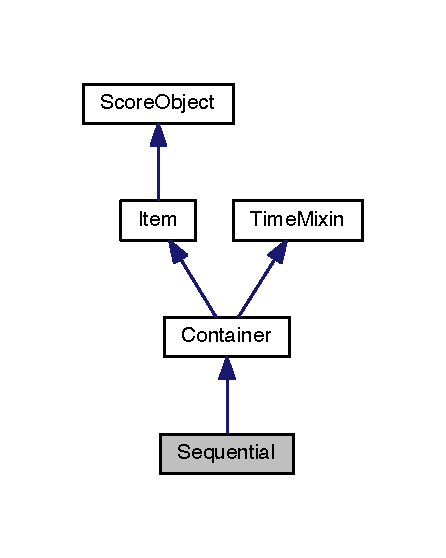
\includegraphics[width=214pt]{class_sequential__inherit__graph}
\end{center}
\end{figure}


Collaboration diagram for Sequential\-:\nopagebreak
\begin{figure}[H]
\begin{center}
\leavevmode
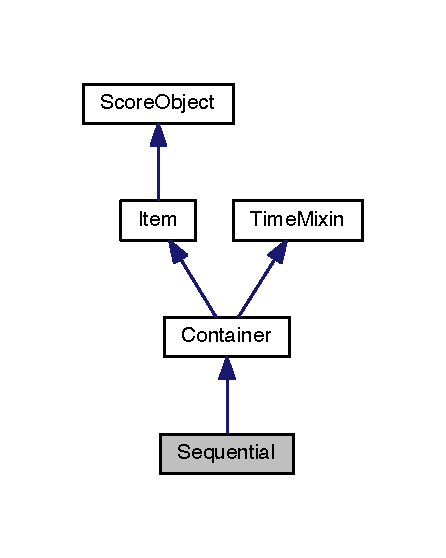
\includegraphics[width=214pt]{class_sequential__coll__graph}
\end{center}
\end{figure}
\subsection*{Public Member Functions}
\begin{DoxyCompactItemize}
\item 
void \hyperlink{class_sequential_aad0311a6dcb3f90c6dd5a397e3fbb7d0}{constrain\-Timing} (void)
\end{DoxyCompactItemize}


\subsection{Detailed Description}
\mbox{[}concrete class\mbox{]} A \hyperlink{class_sequential}{Sequential} expresses that the items contained in it follow each other in a sequential manner in time.

T\-O\-D\-O\-: revise orig Strasheela doc Usually, the parameter end\-Time of a proceeding item equals the parameter start\-Time of the following item. However, setting the parameter offset\-Time of an item to a value greater zero causes a gap (i.\-e. a pause) before the item and a negative offset\-Time causes an overlap with the proceeding item. For a documentation of the time unit see doc of \hyperlink{class_time_mixin}{Time\-Mixin}. N\-B\-: A negative offset\-Time value is not possible if the offset\-Time is a F\-D integer (which presently is the only option). 

\subsection{Member Function Documentation}
\hypertarget{class_sequential_aad0311a6dcb3f90c6dd5a397e3fbb7d0}{\index{Sequential@{Sequential}!constrain\-Timing@{constrain\-Timing}}
\index{constrain\-Timing@{constrain\-Timing}!Sequential@{Sequential}}
\subsubsection[{constrain\-Timing}]{\setlength{\rightskip}{0pt plus 5cm}void Sequential\-::constrain\-Timing (
\begin{DoxyParamCaption}
\item[{void}]{}
\end{DoxyParamCaption}
)}}\label{class_sequential_aad0311a6dcb3f90c6dd5a397e3fbb7d0}


The documentation for this class was generated from the following file\-:\begin{DoxyCompactItemize}
\item 
Music\-Representation/\hyperlink{_score_core___container_8h}{Score\-Core\-\_\-\-Container.\-h}\end{DoxyCompactItemize}

\hypertarget{class_simultaneous}{\section{Simultaneous Class Reference}
\label{class_simultaneous}\index{Simultaneous@{Simultaneous}}
}


{\ttfamily \#include $<$Score\-Core\-\_\-\-Container.\-h$>$}



Inheritance diagram for Simultaneous\-:\nopagebreak
\begin{figure}[H]
\begin{center}
\leavevmode
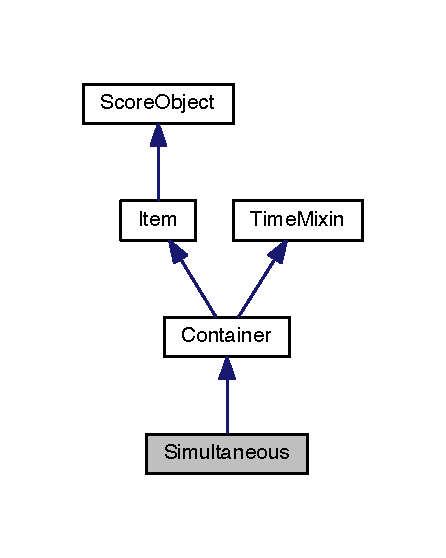
\includegraphics[width=214pt]{class_simultaneous__inherit__graph}
\end{center}
\end{figure}


Collaboration diagram for Simultaneous\-:\nopagebreak
\begin{figure}[H]
\begin{center}
\leavevmode
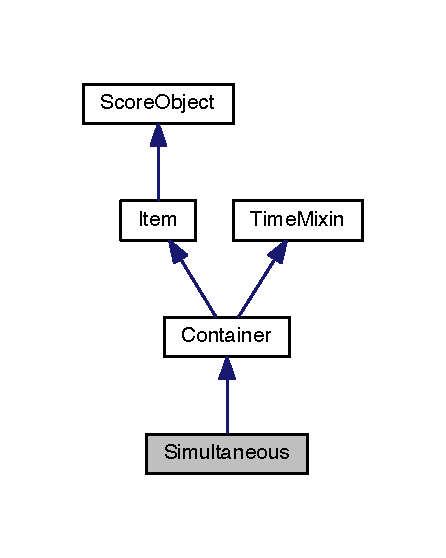
\includegraphics[width=214pt]{class_simultaneous__coll__graph}
\end{center}
\end{figure}
\subsection*{Public Member Functions}
\begin{DoxyCompactItemize}
\item 
void \hyperlink{class_simultaneous_a946e7fb212eb1d3aa2e8812a867b897d}{constrain\-Timing} (void)
\end{DoxyCompactItemize}


\subsection{Detailed Description}
\mbox{[}concrete class\mbox{]} A \hyperlink{class_simultaneous}{Simultaneous} expresses that the items contained in it start at the same time.

However, setting the parameter offset\-Time of an item to a value greater zero causes this item to delay its start\-Time the amount of offset\-Time. For a documentation of the time unit see doc of \hyperlink{class_time_mixin}{Time\-Mixin}. 

\subsection{Member Function Documentation}
\hypertarget{class_simultaneous_a946e7fb212eb1d3aa2e8812a867b897d}{\index{Simultaneous@{Simultaneous}!constrain\-Timing@{constrain\-Timing}}
\index{constrain\-Timing@{constrain\-Timing}!Simultaneous@{Simultaneous}}
\subsubsection[{constrain\-Timing}]{\setlength{\rightskip}{0pt plus 5cm}void Simultaneous\-::constrain\-Timing (
\begin{DoxyParamCaption}
\item[{void}]{}
\end{DoxyParamCaption}
)}}\label{class_simultaneous_a946e7fb212eb1d3aa2e8812a867b897d}


The documentation for this class was generated from the following file\-:\begin{DoxyCompactItemize}
\item 
Music\-Representation/\hyperlink{_score_core___container_8h}{Score\-Core\-\_\-\-Container.\-h}\end{DoxyCompactItemize}

\hypertarget{class_time_interval}{\section{Time\-Interval Class Reference}
\label{class_time_interval}\index{Time\-Interval@{Time\-Interval}}
}


{\ttfamily \#include $<$Score\-Core\-\_\-\-Parameter.\-h$>$}



Inheritance diagram for Time\-Interval\-:\nopagebreak
\begin{figure}[H]
\begin{center}
\leavevmode
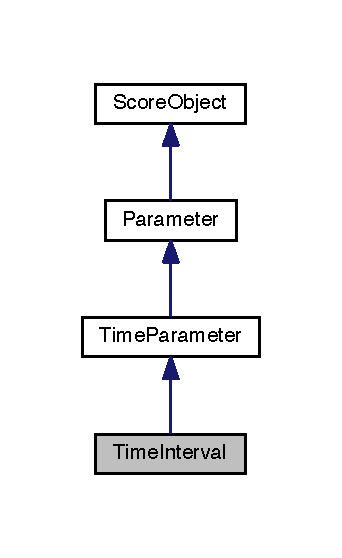
\includegraphics[width=164pt]{class_time_interval__inherit__graph}
\end{center}
\end{figure}


Collaboration diagram for Time\-Interval\-:\nopagebreak
\begin{figure}[H]
\begin{center}
\leavevmode
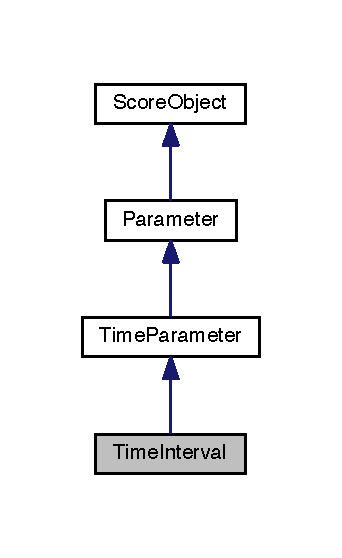
\includegraphics[width=164pt]{class_time_interval__coll__graph}
\end{center}
\end{figure}
\subsection*{Public Member Functions}
\begin{DoxyCompactItemize}
\item 
\hyperlink{class_time_interval_ae82fb340f3698a69622908fa8425dac8}{Time\-Interval} (\hyperlink{_score_core___score_object_8h_ab88aad89d974920ebfb0b0c9e46f61b4}{Args} as)
\end{DoxyCompactItemize}


\subsection{Constructor \& Destructor Documentation}
\hypertarget{class_time_interval_ae82fb340f3698a69622908fa8425dac8}{\index{Time\-Interval@{Time\-Interval}!Time\-Interval@{Time\-Interval}}
\index{Time\-Interval@{Time\-Interval}!TimeInterval@{Time\-Interval}}
\subsubsection[{Time\-Interval}]{\setlength{\rightskip}{0pt plus 5cm}Time\-Interval\-::\-Time\-Interval (
\begin{DoxyParamCaption}
\item[{{\bf Args}}]{as}
\end{DoxyParamCaption}
)\hspace{0.3cm}{\ttfamily [inline]}}}\label{class_time_interval_ae82fb340f3698a69622908fa8425dac8}


The documentation for this class was generated from the following file\-:\begin{DoxyCompactItemize}
\item 
Music\-Representation/\hyperlink{_score_core___parameter_8h}{Score\-Core\-\_\-\-Parameter.\-h}\end{DoxyCompactItemize}

\hypertarget{class_time_mixin}{\section{Time\-Mixin Class Reference}
\label{class_time_mixin}\index{Time\-Mixin@{Time\-Mixin}}
}


{\ttfamily \#include $<$Score\-Core\-\_\-\-Time\-Mixin.\-h$>$}



Inheritance diagram for Time\-Mixin\-:\nopagebreak
\begin{figure}[H]
\begin{center}
\leavevmode
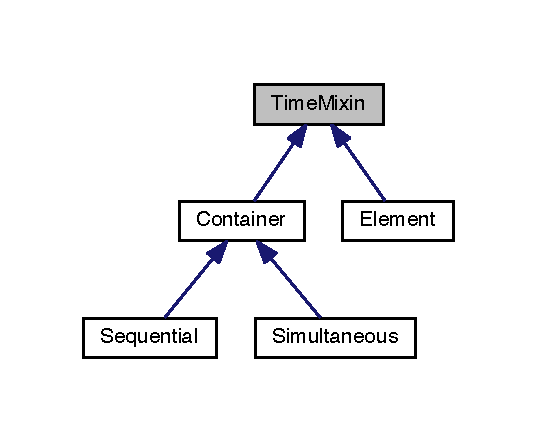
\includegraphics[width=257pt]{class_time_mixin__inherit__graph}
\end{center}
\end{figure}
\subsection*{Public Member Functions}
\begin{DoxyCompactItemize}
\item 
\hyperlink{class_time_mixin_ae9f2a45403a3822b0b41438735ef2bda}{Time\-Mixin} (\hyperlink{_score_core___score_object_8h_ab88aad89d974920ebfb0b0c9e46f61b4}{Args} as)
\item 
int \hyperlink{class_time_mixin_af90ab98a0d498f1e8f233a5d61b07379}{get\-Offset\-Time} (void)
\item 
int \hyperlink{class_time_mixin_a2005478aaa21c3f1603f52b7e9b30cd1}{get\-Start\-Time} (void)
\item 
int \hyperlink{class_time_mixin_af15fb388c632cef74b8454353c202a7e}{get\-Duration} (void)
\item 
int \hyperlink{class_time_mixin_a3704937133fcbc65923fa18089851ccb}{get\-End\-Time} (void)
\item 
\hyperlink{class_time_interval}{Time\-Interval} $\ast$ \hyperlink{class_time_mixin_a078eae46f09af52e60655b6beeda638b}{get\-Offset\-Time\-Parameter} (void)
\item 
\hyperlink{class_time_point}{Time\-Point} $\ast$ \hyperlink{class_time_mixin_adaa5430a2d698f3a353fa4f5e2ed6d9d}{get\-Start\-Time\-Parameter} (void)
\item 
\hyperlink{class_time_interval}{Time\-Interval} $\ast$ \hyperlink{class_time_mixin_aae885e98ca603718ff58d8eb5eb67918}{get\-Duration\-Parameter} (void)
\item 
\hyperlink{class_time_point}{Time\-Point} $\ast$ \hyperlink{class_time_mixin_a52f6b9d308cb3336c28e2053d0ac6004}{get\-End\-Time\-Parameter} (void)
\end{DoxyCompactItemize}


\subsection{Detailed Description}
\mbox{[}abstract class\mbox{]} The \hyperlink{class_time_mixin}{Time\-Mixin} adds several timing attributes and methods to its subclasses. 

\subsection{Constructor \& Destructor Documentation}
\hypertarget{class_time_mixin_ae9f2a45403a3822b0b41438735ef2bda}{\index{Time\-Mixin@{Time\-Mixin}!Time\-Mixin@{Time\-Mixin}}
\index{Time\-Mixin@{Time\-Mixin}!TimeMixin@{Time\-Mixin}}
\subsubsection[{Time\-Mixin}]{\setlength{\rightskip}{0pt plus 5cm}Time\-Mixin\-::\-Time\-Mixin (
\begin{DoxyParamCaption}
\item[{{\bf Args}}]{as}
\end{DoxyParamCaption}
)}}\label{class_time_mixin_ae9f2a45403a3822b0b41438735ef2bda}
\hyperlink{class_time_mixin}{Time\-Mixin} Constructor.

The Args map (later all these ints are replaced by Gecode\-::\-Int\-Var) 
\begin{DoxyParams}{Parameters}
{\em int} & offset\-Time \\
\hline
{\em int} & start\-Time \\
\hline
{\em int} & duration \\
\hline
{\em int} & end\-Time \\
\hline
{\em string} & time\-Unit\\
\hline
\end{DoxyParams}
The instance variables start\-Time and end\-Time are absolute Time\-Points. The variable offset\-Time is a relative \hyperlink{class_time_interval}{Time\-Interval}, whose meaning depends on the enclosign container (semultaneous or sequential). The variable duration is the \hyperlink{class_time_interval}{Time\-Interval} difference between start\-Time and end\-Time.

The time\-Unit specifies what the numeric values for the values of the parameters like start\-Time and end\-Time actually mean. The time\-Unit either specifies an absolute value (e.\-g., \char`\"{}seconds\char`\"{}) or a relative value (e.\-g., \char`\"{}beats\char`\"{}). The meaning of a beat depends on the output definition. For instance, it may mean a quarter note. T\-O\-D\-O\-: update doc -- this is still the Strasheela doc, until these value conversions are actually implemented Currently, possible values are 'seconds' (or 'secs'), 'milliseconds' (or 'msecs'), 'beats', or beats(\-N), where N means number of ticks (i.\-e. the integer range) within a beat. For example, if the time\-Unit = beats(4) and a beat corresponds to a quarter note, then a note of duration 1 corresponds to a sixteenth note. beats is equivalent with beats(1). The meaning of a beat for sound output can be specified by the tempo (see Init.\-set\-Beat\-Duration, Init.\-set\-Tempo etc.)

N\-B\-: To avoid confusion, the time\-Unit of all temporal items in the score are unified when a score is created. 

\subsection{Member Function Documentation}
\hypertarget{class_time_mixin_af15fb388c632cef74b8454353c202a7e}{\index{Time\-Mixin@{Time\-Mixin}!get\-Duration@{get\-Duration}}
\index{get\-Duration@{get\-Duration}!TimeMixin@{Time\-Mixin}}
\subsubsection[{get\-Duration}]{\setlength{\rightskip}{0pt plus 5cm}int Time\-Mixin\-::get\-Duration (
\begin{DoxyParamCaption}
\item[{void}]{}
\end{DoxyParamCaption}
)\hspace{0.3cm}{\ttfamily [inline]}}}\label{class_time_mixin_af15fb388c632cef74b8454353c202a7e}
\hypertarget{class_time_mixin_aae885e98ca603718ff58d8eb5eb67918}{\index{Time\-Mixin@{Time\-Mixin}!get\-Duration\-Parameter@{get\-Duration\-Parameter}}
\index{get\-Duration\-Parameter@{get\-Duration\-Parameter}!TimeMixin@{Time\-Mixin}}
\subsubsection[{get\-Duration\-Parameter}]{\setlength{\rightskip}{0pt plus 5cm}{\bf Time\-Interval}$\ast$ Time\-Mixin\-::get\-Duration\-Parameter (
\begin{DoxyParamCaption}
\item[{void}]{}
\end{DoxyParamCaption}
)\hspace{0.3cm}{\ttfamily [inline]}}}\label{class_time_mixin_aae885e98ca603718ff58d8eb5eb67918}
\hypertarget{class_time_mixin_a3704937133fcbc65923fa18089851ccb}{\index{Time\-Mixin@{Time\-Mixin}!get\-End\-Time@{get\-End\-Time}}
\index{get\-End\-Time@{get\-End\-Time}!TimeMixin@{Time\-Mixin}}
\subsubsection[{get\-End\-Time}]{\setlength{\rightskip}{0pt plus 5cm}int Time\-Mixin\-::get\-End\-Time (
\begin{DoxyParamCaption}
\item[{void}]{}
\end{DoxyParamCaption}
)\hspace{0.3cm}{\ttfamily [inline]}}}\label{class_time_mixin_a3704937133fcbc65923fa18089851ccb}
\hypertarget{class_time_mixin_a52f6b9d308cb3336c28e2053d0ac6004}{\index{Time\-Mixin@{Time\-Mixin}!get\-End\-Time\-Parameter@{get\-End\-Time\-Parameter}}
\index{get\-End\-Time\-Parameter@{get\-End\-Time\-Parameter}!TimeMixin@{Time\-Mixin}}
\subsubsection[{get\-End\-Time\-Parameter}]{\setlength{\rightskip}{0pt plus 5cm}{\bf Time\-Point}$\ast$ Time\-Mixin\-::get\-End\-Time\-Parameter (
\begin{DoxyParamCaption}
\item[{void}]{}
\end{DoxyParamCaption}
)\hspace{0.3cm}{\ttfamily [inline]}}}\label{class_time_mixin_a52f6b9d308cb3336c28e2053d0ac6004}
\hypertarget{class_time_mixin_af90ab98a0d498f1e8f233a5d61b07379}{\index{Time\-Mixin@{Time\-Mixin}!get\-Offset\-Time@{get\-Offset\-Time}}
\index{get\-Offset\-Time@{get\-Offset\-Time}!TimeMixin@{Time\-Mixin}}
\subsubsection[{get\-Offset\-Time}]{\setlength{\rightskip}{0pt plus 5cm}int Time\-Mixin\-::get\-Offset\-Time (
\begin{DoxyParamCaption}
\item[{void}]{}
\end{DoxyParamCaption}
)\hspace{0.3cm}{\ttfamily [inline]}}}\label{class_time_mixin_af90ab98a0d498f1e8f233a5d61b07379}
\hypertarget{class_time_mixin_a078eae46f09af52e60655b6beeda638b}{\index{Time\-Mixin@{Time\-Mixin}!get\-Offset\-Time\-Parameter@{get\-Offset\-Time\-Parameter}}
\index{get\-Offset\-Time\-Parameter@{get\-Offset\-Time\-Parameter}!TimeMixin@{Time\-Mixin}}
\subsubsection[{get\-Offset\-Time\-Parameter}]{\setlength{\rightskip}{0pt plus 5cm}{\bf Time\-Interval}$\ast$ Time\-Mixin\-::get\-Offset\-Time\-Parameter (
\begin{DoxyParamCaption}
\item[{void}]{}
\end{DoxyParamCaption}
)\hspace{0.3cm}{\ttfamily [inline]}}}\label{class_time_mixin_a078eae46f09af52e60655b6beeda638b}
\hypertarget{class_time_mixin_a2005478aaa21c3f1603f52b7e9b30cd1}{\index{Time\-Mixin@{Time\-Mixin}!get\-Start\-Time@{get\-Start\-Time}}
\index{get\-Start\-Time@{get\-Start\-Time}!TimeMixin@{Time\-Mixin}}
\subsubsection[{get\-Start\-Time}]{\setlength{\rightskip}{0pt plus 5cm}int Time\-Mixin\-::get\-Start\-Time (
\begin{DoxyParamCaption}
\item[{void}]{}
\end{DoxyParamCaption}
)\hspace{0.3cm}{\ttfamily [inline]}}}\label{class_time_mixin_a2005478aaa21c3f1603f52b7e9b30cd1}
\hypertarget{class_time_mixin_adaa5430a2d698f3a353fa4f5e2ed6d9d}{\index{Time\-Mixin@{Time\-Mixin}!get\-Start\-Time\-Parameter@{get\-Start\-Time\-Parameter}}
\index{get\-Start\-Time\-Parameter@{get\-Start\-Time\-Parameter}!TimeMixin@{Time\-Mixin}}
\subsubsection[{get\-Start\-Time\-Parameter}]{\setlength{\rightskip}{0pt plus 5cm}{\bf Time\-Point}$\ast$ Time\-Mixin\-::get\-Start\-Time\-Parameter (
\begin{DoxyParamCaption}
\item[{void}]{}
\end{DoxyParamCaption}
)\hspace{0.3cm}{\ttfamily [inline]}}}\label{class_time_mixin_adaa5430a2d698f3a353fa4f5e2ed6d9d}


The documentation for this class was generated from the following files\-:\begin{DoxyCompactItemize}
\item 
Music\-Representation/\hyperlink{_score_core___time_mixin_8h}{Score\-Core\-\_\-\-Time\-Mixin.\-h}\item 
Music\-Representation/\hyperlink{_score_core___time_mixin_8cpp}{Score\-Core\-\_\-\-Time\-Mixin.\-cpp}\end{DoxyCompactItemize}

\hypertarget{class_time_parameter}{\section{Time\-Parameter Class Reference}
\label{class_time_parameter}\index{Time\-Parameter@{Time\-Parameter}}
}


{\ttfamily \#include $<$Score\-Core\-\_\-\-Parameter.\-h$>$}



Inheritance diagram for Time\-Parameter\-:\nopagebreak
\begin{figure}[H]
\begin{center}
\leavevmode
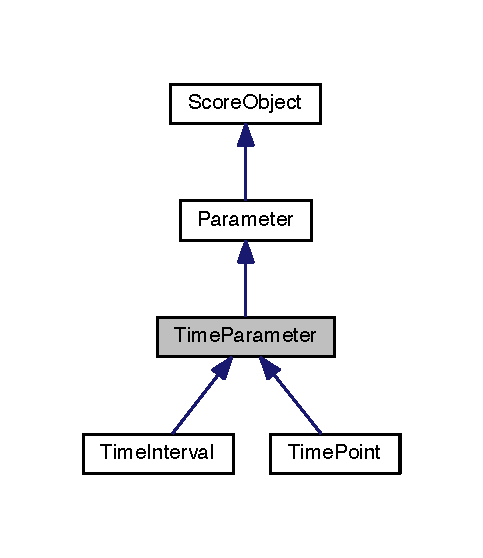
\includegraphics[width=232pt]{class_time_parameter__inherit__graph}
\end{center}
\end{figure}


Collaboration diagram for Time\-Parameter\-:\nopagebreak
\begin{figure}[H]
\begin{center}
\leavevmode
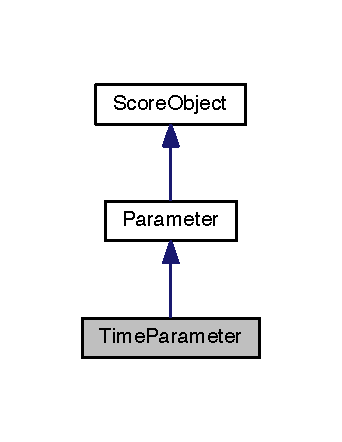
\includegraphics[width=164pt]{class_time_parameter__coll__graph}
\end{center}
\end{figure}
\subsection*{Public Member Functions}
\begin{DoxyCompactItemize}
\item 
\hyperlink{class_time_parameter_acb1797eda1cb8172b4bfd10be1e3c82d}{Time\-Parameter} (\hyperlink{_score_core___score_object_8h_ab88aad89d974920ebfb0b0c9e46f61b4}{Args} as)
\item 
float \hyperlink{class_time_parameter_ac520983d7bc0c3e76ab2dd0c390a10f4}{get\-Value\-In\-Seconds} (void)
\item 
float \hyperlink{class_time_parameter_a9e8cee5a439d58f355b6fa0e2e453036}{get\-Value\-In\-Beats} (void)
\end{DoxyCompactItemize}


\subsection{Constructor \& Destructor Documentation}
\hypertarget{class_time_parameter_acb1797eda1cb8172b4bfd10be1e3c82d}{\index{Time\-Parameter@{Time\-Parameter}!Time\-Parameter@{Time\-Parameter}}
\index{Time\-Parameter@{Time\-Parameter}!TimeParameter@{Time\-Parameter}}
\subsubsection[{Time\-Parameter}]{\setlength{\rightskip}{0pt plus 5cm}Time\-Parameter\-::\-Time\-Parameter (
\begin{DoxyParamCaption}
\item[{{\bf Args}}]{as}
\end{DoxyParamCaption}
)\hspace{0.3cm}{\ttfamily [inline]}}}\label{class_time_parameter_acb1797eda1cb8172b4bfd10be1e3c82d}


\subsection{Member Function Documentation}
\hypertarget{class_time_parameter_a9e8cee5a439d58f355b6fa0e2e453036}{\index{Time\-Parameter@{Time\-Parameter}!get\-Value\-In\-Beats@{get\-Value\-In\-Beats}}
\index{get\-Value\-In\-Beats@{get\-Value\-In\-Beats}!TimeParameter@{Time\-Parameter}}
\subsubsection[{get\-Value\-In\-Beats}]{\setlength{\rightskip}{0pt plus 5cm}float Time\-Parameter\-::get\-Value\-In\-Beats (
\begin{DoxyParamCaption}
\item[{void}]{}
\end{DoxyParamCaption}
)}}\label{class_time_parameter_a9e8cee5a439d58f355b6fa0e2e453036}
\hypertarget{class_time_parameter_ac520983d7bc0c3e76ab2dd0c390a10f4}{\index{Time\-Parameter@{Time\-Parameter}!get\-Value\-In\-Seconds@{get\-Value\-In\-Seconds}}
\index{get\-Value\-In\-Seconds@{get\-Value\-In\-Seconds}!TimeParameter@{Time\-Parameter}}
\subsubsection[{get\-Value\-In\-Seconds}]{\setlength{\rightskip}{0pt plus 5cm}float Time\-Parameter\-::get\-Value\-In\-Seconds (
\begin{DoxyParamCaption}
\item[{void}]{}
\end{DoxyParamCaption}
)}}\label{class_time_parameter_ac520983d7bc0c3e76ab2dd0c390a10f4}


The documentation for this class was generated from the following file\-:\begin{DoxyCompactItemize}
\item 
Music\-Representation/\hyperlink{_score_core___parameter_8h}{Score\-Core\-\_\-\-Parameter.\-h}\end{DoxyCompactItemize}

\hypertarget{class_time_point}{\section{Time\-Point Class Reference}
\label{class_time_point}\index{Time\-Point@{Time\-Point}}
}


{\ttfamily \#include $<$Score\-Core\-\_\-\-Parameter.\-h$>$}



Inheritance diagram for Time\-Point\-:\nopagebreak
\begin{figure}[H]
\begin{center}
\leavevmode
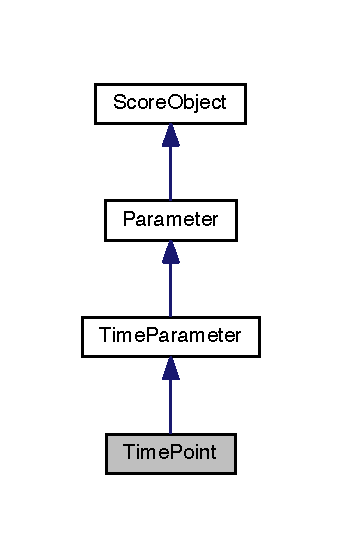
\includegraphics[width=164pt]{class_time_point__inherit__graph}
\end{center}
\end{figure}


Collaboration diagram for Time\-Point\-:\nopagebreak
\begin{figure}[H]
\begin{center}
\leavevmode
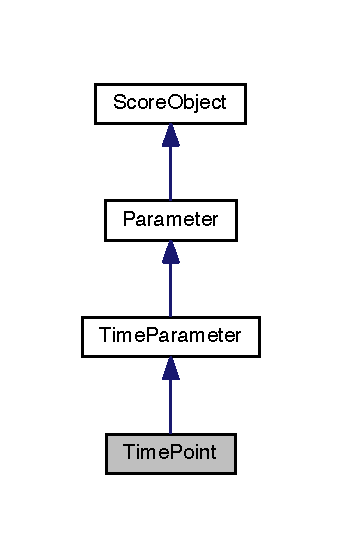
\includegraphics[width=164pt]{class_time_point__coll__graph}
\end{center}
\end{figure}
\subsection*{Public Member Functions}
\begin{DoxyCompactItemize}
\item 
\hyperlink{class_time_point_a6dedd66d04e1da02f98d240b8eccebcd}{Time\-Point} (\hyperlink{_score_core___score_object_8h_ab88aad89d974920ebfb0b0c9e46f61b4}{Args} as)
\end{DoxyCompactItemize}


\subsection{Constructor \& Destructor Documentation}
\hypertarget{class_time_point_a6dedd66d04e1da02f98d240b8eccebcd}{\index{Time\-Point@{Time\-Point}!Time\-Point@{Time\-Point}}
\index{Time\-Point@{Time\-Point}!TimePoint@{Time\-Point}}
\subsubsection[{Time\-Point}]{\setlength{\rightskip}{0pt plus 5cm}Time\-Point\-::\-Time\-Point (
\begin{DoxyParamCaption}
\item[{{\bf Args}}]{as}
\end{DoxyParamCaption}
)\hspace{0.3cm}{\ttfamily [inline]}}}\label{class_time_point_a6dedd66d04e1da02f98d240b8eccebcd}


The documentation for this class was generated from the following file\-:\begin{DoxyCompactItemize}
\item 
Music\-Representation/\hyperlink{_score_core___parameter_8h}{Score\-Core\-\_\-\-Parameter.\-h}\end{DoxyCompactItemize}

\chapter{File Documentation}
\hypertarget{main_8cpp}{\section{Music\-Representation/main.cpp File Reference}
\label{main_8cpp}\index{Music\-Representation/main.\-cpp@{Music\-Representation/main.\-cpp}}
}
{\ttfamily \#include \char`\"{}Music\-Utils.\-h\char`\"{}}\\*
{\ttfamily \#include \char`\"{}Score\-Core\-\_\-\-Element.\-h\char`\"{}}\\*
Include dependency graph for main.\-cpp\-:\nopagebreak
\begin{figure}[H]
\begin{center}
\leavevmode
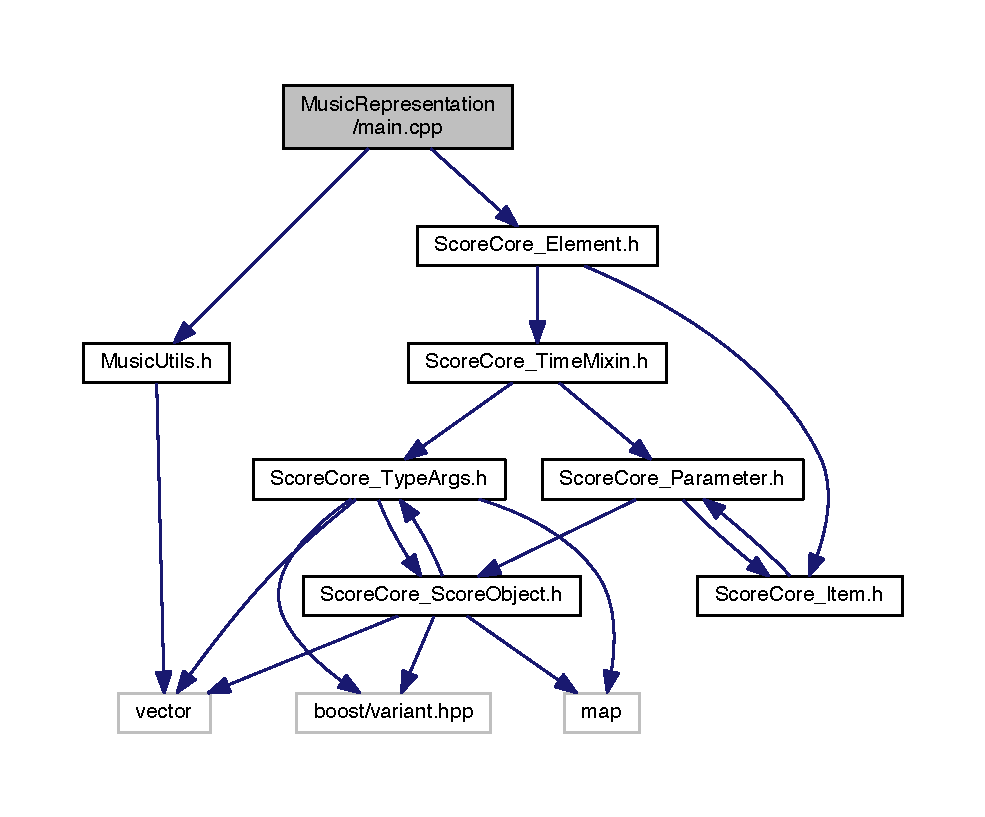
\includegraphics[width=350pt]{main_8cpp__incl}
\end{center}
\end{figure}
\subsection*{Functions}
\begin{DoxyCompactItemize}
\item 
int \hyperlink{main_8cpp_ac0f2228420376f4db7e1274f2b41667c}{main} (int argc, const char $\ast$argv\mbox{[}$\,$\mbox{]})
\end{DoxyCompactItemize}


\subsection{Function Documentation}
\hypertarget{main_8cpp_ac0f2228420376f4db7e1274f2b41667c}{\index{main.\-cpp@{main.\-cpp}!main@{main}}
\index{main@{main}!main.cpp@{main.\-cpp}}
\subsubsection[{main}]{\setlength{\rightskip}{0pt plus 5cm}int main (
\begin{DoxyParamCaption}
\item[{int}]{argc, }
\item[{const char $\ast$}]{argv\mbox{[}$\,$\mbox{]}}
\end{DoxyParamCaption}
)}}\label{main_8cpp_ac0f2228420376f4db7e1274f2b41667c}

\hypertarget{_music_utils_8cpp}{\section{Music\-Representation/\-Music\-Utils.cpp File Reference}
\label{_music_utils_8cpp}\index{Music\-Representation/\-Music\-Utils.\-cpp@{Music\-Representation/\-Music\-Utils.\-cpp}}
}
{\ttfamily \#include $<$math.\-h$>$}\\*
{\ttfamily \#include $<$string$>$}\\*
{\ttfamily \#include $<$boost/algorithm/string/predicate.\-hpp$>$}\\*
{\ttfamily \#include \char`\"{}Music\-Utils.\-h\char`\"{}}\\*
Include dependency graph for Music\-Utils.\-cpp\-:\nopagebreak
\begin{figure}[H]
\begin{center}
\leavevmode
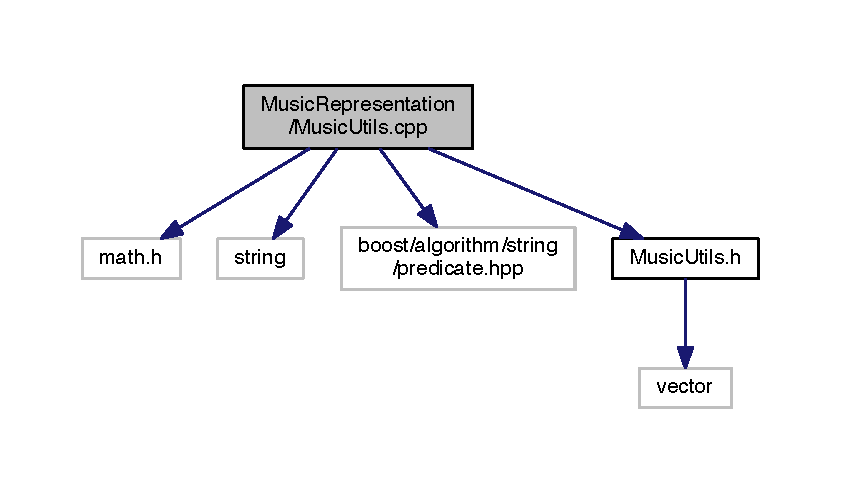
\includegraphics[width=350pt]{_music_utils_8cpp__incl}
\end{center}
\end{figure}
\subsection*{Functions}
\begin{DoxyCompactItemize}
\item 
double \hyperlink{_music_utils_8cpp_a4e90125986c69efb65d203f629861b2c}{keynum\-To\-Freq} (double keynum, int keys\-Per\-Octave)
\item 
double \hyperlink{_music_utils_8cpp_a0202a39d2949226eb55871bed5d0a4eb}{freq\-To\-Keynum} (double freq, int keys\-Per\-Octave)
\item 
bool \hyperlink{_music_utils_8cpp_ad4c78be5ecfdffb6fceb4007e2095a5f}{is\-E\-T} (std\-::string pitch\-Unit)
\item 
int \hyperlink{_music_utils_8cpp_a83b63f5637bb283b9511cc754a9b0a56}{get\-Pitches\-Per\-Octave} (std\-::string pitch\-Unit)
\item 
double \hyperlink{_music_utils_8cpp_a69504725fd34c3556d3e22869c17ffdc}{pitch\-To\-Midi} (double pitch, std\-::string pitch\-Unit)
\end{DoxyCompactItemize}
\subsection*{Variables}
\begin{DoxyCompactItemize}
\item 
const float \hyperlink{_music_utils_8cpp_a2b485959ae284e5a6d7caca4732262a1}{freq0} = 8.\-175798915643707
\end{DoxyCompactItemize}


\subsection{Detailed Description}
This file defines some utilities which are related to music or acoustics. 

\subsection{Function Documentation}
\hypertarget{_music_utils_8cpp_a0202a39d2949226eb55871bed5d0a4eb}{\index{Music\-Utils.\-cpp@{Music\-Utils.\-cpp}!freq\-To\-Keynum@{freq\-To\-Keynum}}
\index{freq\-To\-Keynum@{freq\-To\-Keynum}!MusicUtils.cpp@{Music\-Utils.\-cpp}}
\subsubsection[{freq\-To\-Keynum}]{\setlength{\rightskip}{0pt plus 5cm}double freq\-To\-Keynum (
\begin{DoxyParamCaption}
\item[{double}]{freq, }
\item[{int}]{keys\-Per\-Octave}
\end{DoxyParamCaption}
)}}\label{_music_utils_8cpp_a0202a39d2949226eb55871bed5d0a4eb}
Transforms freq into the corresponding keynum in an equally tempered scale with keys\-Per\-Octave keys per octave. The function is 'tuned' such that freq\-To\-Keynum(440, 12) returns 69. Note that he term keynum here is not limited to a M\-I\-D\-I keynumber but denotes a keynumber in any equidistant tuning. For instance, if keys\-Per\-Octave=1200 then keynum denotes cent values. \hypertarget{_music_utils_8cpp_a83b63f5637bb283b9511cc754a9b0a56}{\index{Music\-Utils.\-cpp@{Music\-Utils.\-cpp}!get\-Pitches\-Per\-Octave@{get\-Pitches\-Per\-Octave}}
\index{get\-Pitches\-Per\-Octave@{get\-Pitches\-Per\-Octave}!MusicUtils.cpp@{Music\-Utils.\-cpp}}
\subsubsection[{get\-Pitches\-Per\-Octave}]{\setlength{\rightskip}{0pt plus 5cm}int get\-Pitches\-Per\-Octave (
\begin{DoxyParamCaption}
\item[{std\-::string}]{pitch\-Unit}
\end{DoxyParamCaption}
)}}\label{_music_utils_8cpp_a83b63f5637bb283b9511cc754a9b0a56}
Returns the pitches per octave expressed by an E\-T pitch unit, e.\-g., for et31 it returns 31. \hypertarget{_music_utils_8cpp_ad4c78be5ecfdffb6fceb4007e2095a5f}{\index{Music\-Utils.\-cpp@{Music\-Utils.\-cpp}!is\-E\-T@{is\-E\-T}}
\index{is\-E\-T@{is\-E\-T}!MusicUtils.cpp@{Music\-Utils.\-cpp}}
\subsubsection[{is\-E\-T}]{\setlength{\rightskip}{0pt plus 5cm}bool is\-E\-T (
\begin{DoxyParamCaption}
\item[{std\-::string}]{pitch\-Unit}
\end{DoxyParamCaption}
)}}\label{_music_utils_8cpp_ad4c78be5ecfdffb6fceb4007e2095a5f}
Returns true if Pitch\-Unit is an atom which matches the pattern et$<$\-Digit$>$+ such as et31 or et72. \hypertarget{_music_utils_8cpp_a4e90125986c69efb65d203f629861b2c}{\index{Music\-Utils.\-cpp@{Music\-Utils.\-cpp}!keynum\-To\-Freq@{keynum\-To\-Freq}}
\index{keynum\-To\-Freq@{keynum\-To\-Freq}!MusicUtils.cpp@{Music\-Utils.\-cpp}}
\subsubsection[{keynum\-To\-Freq}]{\setlength{\rightskip}{0pt plus 5cm}double keynum\-To\-Freq (
\begin{DoxyParamCaption}
\item[{double}]{keynum, }
\item[{int}]{keys\-Per\-Octave}
\end{DoxyParamCaption}
)}}\label{_music_utils_8cpp_a4e90125986c69efb65d203f629861b2c}
Transforms a keynum into the corresponding frequency in an equally tempered scale with keys\-Per\-Octave keys per octave. The function is 'tuned' such that keynum\-To\-Freq(69 12) returns 440 Hz. Note that he term keynum here is not limited to a M\-I\-D\-I keynumber but denotes a keynumber in any equidistant tuning. For instance, if keys\-Per\-Octave=1200 then keynum denotes cent values. \hypertarget{_music_utils_8cpp_a69504725fd34c3556d3e22869c17ffdc}{\index{Music\-Utils.\-cpp@{Music\-Utils.\-cpp}!pitch\-To\-Midi@{pitch\-To\-Midi}}
\index{pitch\-To\-Midi@{pitch\-To\-Midi}!MusicUtils.cpp@{Music\-Utils.\-cpp}}
\subsubsection[{pitch\-To\-Midi}]{\setlength{\rightskip}{0pt plus 5cm}double pitch\-To\-Midi (
\begin{DoxyParamCaption}
\item[{double}]{pitch, }
\item[{std\-::string}]{pitch\-Unit}
\end{DoxyParamCaption}
)}}\label{_music_utils_8cpp_a69504725fd34c3556d3e22869c17ffdc}
Transforms pitch, measured in pitch\-Unit, into the corresponding \char`\"{}\-Midi float\char`\"{}

A \char`\"{}\-Midi float\char`\"{} is a Midi number where positions after the decimal point express microtonal pitch deviations (e.\-g., 60.\-5 is middle C raised by a quarter tone). Possible pitch units are \char`\"{}midi\-: (i.\-e., 12-\/\-T\-E\-T); \char`\"{}midicent\char`\"{} or \char`\"{}midic\char`\"{} (pitch measured in cent); \char`\"{}frequency\char`\"{}, \char`\"{}freq\char`\"{}, \char`\"{}Hz\char`\"{} or \char`\"{}hz\char`\"{} (a frequency measured in Hz); \char`\"{}m\-Hz\char`\"{}; and arbitrary equal temperaments notated \char`\"{}et$<$division\-Of\-Octave$>$\char`\"{}, e.\-g., \char`\"{}et31\char`\"{}, \char`\"{}et72" etc. 

\subsection{Variable Documentation}
\hypertarget{_music_utils_8cpp_a2b485959ae284e5a6d7caca4732262a1}{\index{Music\-Utils.\-cpp@{Music\-Utils.\-cpp}!freq0@{freq0}}
\index{freq0@{freq0}!MusicUtils.cpp@{Music\-Utils.\-cpp}}
\subsubsection[{freq0}]{\setlength{\rightskip}{0pt plus 5cm}const float freq0 = 8.\-175798915643707}}\label{_music_utils_8cpp_a2b485959ae284e5a6d7caca4732262a1}
freq at keynum 0, keynum 69 = 440 Hz 
\hypertarget{_music_utils_8h}{\section{Music\-Representation/\-Music\-Utils.h File Reference}
\label{_music_utils_8h}\index{Music\-Representation/\-Music\-Utils.\-h@{Music\-Representation/\-Music\-Utils.\-h}}
}
{\ttfamily \#include $<$vector$>$}\\*
Include dependency graph for Music\-Utils.\-h\-:\nopagebreak
\begin{figure}[H]
\begin{center}
\leavevmode
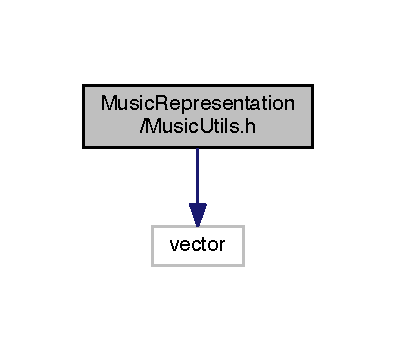
\includegraphics[width=190pt]{_music_utils_8h__incl}
\end{center}
\end{figure}
This graph shows which files directly or indirectly include this file\-:\nopagebreak
\begin{figure}[H]
\begin{center}
\leavevmode
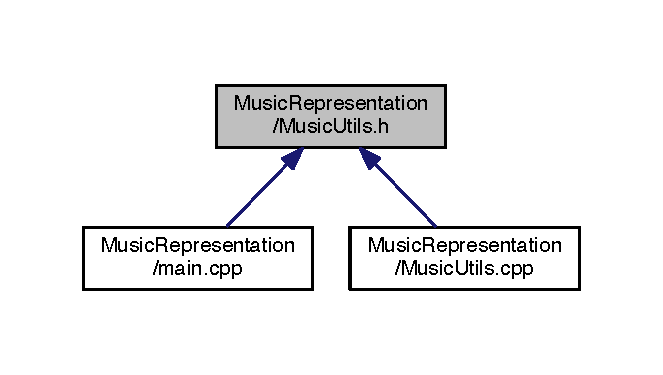
\includegraphics[width=318pt]{_music_utils_8h__dep__incl}
\end{center}
\end{figure}
\subsection*{Functions}
\begin{DoxyCompactItemize}
\item 
double \hyperlink{_music_utils_8h_a4e90125986c69efb65d203f629861b2c}{keynum\-To\-Freq} (double keynum, int keys\-Per\-Octave)
\item 
double \hyperlink{_music_utils_8h_a0202a39d2949226eb55871bed5d0a4eb}{freq\-To\-Keynum} (double freq, int keys\-Per\-Octave)
\item 
bool \hyperlink{_music_utils_8h_ad4c78be5ecfdffb6fceb4007e2095a5f}{is\-E\-T} (std\-::string pitch\-Unit)
\item 
int \hyperlink{_music_utils_8h_a83b63f5637bb283b9511cc754a9b0a56}{get\-Pitches\-Per\-Octave} (std\-::string pitch\-Unit)
\item 
double \hyperlink{_music_utils_8h_a69504725fd34c3556d3e22869c17ffdc}{pitch\-To\-Midi} (double pitch, std\-::string pitch\-Unit)
\end{DoxyCompactItemize}


\subsection{Function Documentation}
\hypertarget{_music_utils_8h_a0202a39d2949226eb55871bed5d0a4eb}{\index{Music\-Utils.\-h@{Music\-Utils.\-h}!freq\-To\-Keynum@{freq\-To\-Keynum}}
\index{freq\-To\-Keynum@{freq\-To\-Keynum}!MusicUtils.h@{Music\-Utils.\-h}}
\subsubsection[{freq\-To\-Keynum}]{\setlength{\rightskip}{0pt plus 5cm}double freq\-To\-Keynum (
\begin{DoxyParamCaption}
\item[{double}]{freq, }
\item[{int}]{keys\-Per\-Octave}
\end{DoxyParamCaption}
)}}\label{_music_utils_8h_a0202a39d2949226eb55871bed5d0a4eb}
Transforms freq into the corresponding keynum in an equally tempered scale with keys\-Per\-Octave keys per octave. The function is 'tuned' such that freq\-To\-Keynum(440, 12) returns 69. Note that he term keynum here is not limited to a M\-I\-D\-I keynumber but denotes a keynumber in any equidistant tuning. For instance, if keys\-Per\-Octave=1200 then keynum denotes cent values. \hypertarget{_music_utils_8h_a83b63f5637bb283b9511cc754a9b0a56}{\index{Music\-Utils.\-h@{Music\-Utils.\-h}!get\-Pitches\-Per\-Octave@{get\-Pitches\-Per\-Octave}}
\index{get\-Pitches\-Per\-Octave@{get\-Pitches\-Per\-Octave}!MusicUtils.h@{Music\-Utils.\-h}}
\subsubsection[{get\-Pitches\-Per\-Octave}]{\setlength{\rightskip}{0pt plus 5cm}int get\-Pitches\-Per\-Octave (
\begin{DoxyParamCaption}
\item[{std\-::string}]{pitch\-Unit}
\end{DoxyParamCaption}
)}}\label{_music_utils_8h_a83b63f5637bb283b9511cc754a9b0a56}
Returns the pitches per octave expressed by an E\-T pitch unit, e.\-g., for et31 it returns 31. \hypertarget{_music_utils_8h_ad4c78be5ecfdffb6fceb4007e2095a5f}{\index{Music\-Utils.\-h@{Music\-Utils.\-h}!is\-E\-T@{is\-E\-T}}
\index{is\-E\-T@{is\-E\-T}!MusicUtils.h@{Music\-Utils.\-h}}
\subsubsection[{is\-E\-T}]{\setlength{\rightskip}{0pt plus 5cm}bool is\-E\-T (
\begin{DoxyParamCaption}
\item[{std\-::string}]{pitch\-Unit}
\end{DoxyParamCaption}
)}}\label{_music_utils_8h_ad4c78be5ecfdffb6fceb4007e2095a5f}
Returns true if Pitch\-Unit is an atom which matches the pattern et$<$\-Digit$>$+ such as et31 or et72. \hypertarget{_music_utils_8h_a4e90125986c69efb65d203f629861b2c}{\index{Music\-Utils.\-h@{Music\-Utils.\-h}!keynum\-To\-Freq@{keynum\-To\-Freq}}
\index{keynum\-To\-Freq@{keynum\-To\-Freq}!MusicUtils.h@{Music\-Utils.\-h}}
\subsubsection[{keynum\-To\-Freq}]{\setlength{\rightskip}{0pt plus 5cm}double keynum\-To\-Freq (
\begin{DoxyParamCaption}
\item[{double}]{keynum, }
\item[{int}]{keys\-Per\-Octave}
\end{DoxyParamCaption}
)}}\label{_music_utils_8h_a4e90125986c69efb65d203f629861b2c}
Transforms a keynum into the corresponding frequency in an equally tempered scale with keys\-Per\-Octave keys per octave. The function is 'tuned' such that keynum\-To\-Freq(69 12) returns 440 Hz. Note that he term keynum here is not limited to a M\-I\-D\-I keynumber but denotes a keynumber in any equidistant tuning. For instance, if keys\-Per\-Octave=1200 then keynum denotes cent values. \hypertarget{_music_utils_8h_a69504725fd34c3556d3e22869c17ffdc}{\index{Music\-Utils.\-h@{Music\-Utils.\-h}!pitch\-To\-Midi@{pitch\-To\-Midi}}
\index{pitch\-To\-Midi@{pitch\-To\-Midi}!MusicUtils.h@{Music\-Utils.\-h}}
\subsubsection[{pitch\-To\-Midi}]{\setlength{\rightskip}{0pt plus 5cm}double pitch\-To\-Midi (
\begin{DoxyParamCaption}
\item[{double}]{pitch, }
\item[{std\-::string}]{pitch\-Unit}
\end{DoxyParamCaption}
)}}\label{_music_utils_8h_a69504725fd34c3556d3e22869c17ffdc}
Transforms pitch, measured in pitch\-Unit, into the corresponding \char`\"{}\-Midi float\char`\"{}

A \char`\"{}\-Midi float\char`\"{} is a Midi number where positions after the decimal point express microtonal pitch deviations (e.\-g., 60.\-5 is middle C raised by a quarter tone). Possible pitch units are \char`\"{}midi\-: (i.\-e., 12-\/\-T\-E\-T); \char`\"{}midicent\char`\"{} or \char`\"{}midic\char`\"{} (pitch measured in cent); \char`\"{}frequency\char`\"{}, \char`\"{}freq\char`\"{}, \char`\"{}Hz\char`\"{} or \char`\"{}hz\char`\"{} (a frequency measured in Hz); \char`\"{}m\-Hz\char`\"{}; and arbitrary equal temperaments notated \char`\"{}et$<$division\-Of\-Octave$>$\char`\"{}, e.\-g., \char`\"{}et31\char`\"{}, \char`\"{}et72" etc. 
\hypertarget{_score_core_8cpp}{\section{Music\-Representation/\-Score\-Core.cpp File Reference}
\label{_score_core_8cpp}\index{Music\-Representation/\-Score\-Core.\-cpp@{Music\-Representation/\-Score\-Core.\-cpp}}
}
{\ttfamily \#include \char`\"{}Score\-Core.\-h\char`\"{}}\\*
Include dependency graph for Score\-Core.\-cpp\-:\nopagebreak
\begin{figure}[H]
\begin{center}
\leavevmode
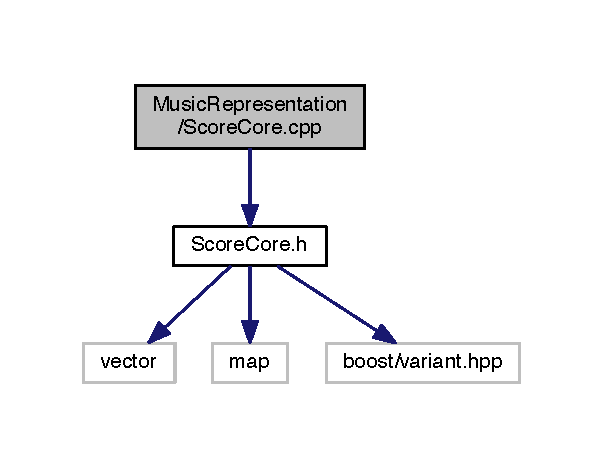
\includegraphics[width=289pt]{_score_core_8cpp__incl}
\end{center}
\end{figure}

\hypertarget{_score_core_8h}{\section{Music\-Representation/\-Score\-Core.h File Reference}
\label{_score_core_8h}\index{Music\-Representation/\-Score\-Core.\-h@{Music\-Representation/\-Score\-Core.\-h}}
}
{\ttfamily \#include $<$vector$>$}\\*
{\ttfamily \#include $<$map$>$}\\*
{\ttfamily \#include $<$boost/variant.\-hpp$>$}\\*
Include dependency graph for Score\-Core.\-h\-:\nopagebreak
\begin{figure}[H]
\begin{center}
\leavevmode
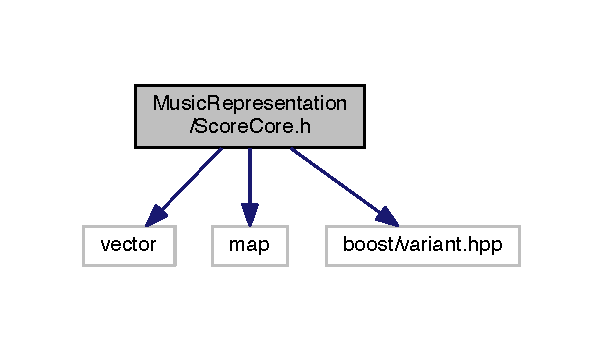
\includegraphics[width=289pt]{_score_core_8h__incl}
\end{center}
\end{figure}
This graph shows which files directly or indirectly include this file\-:\nopagebreak
\begin{figure}[H]
\begin{center}
\leavevmode
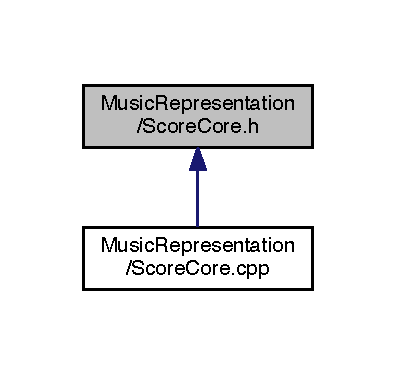
\includegraphics[width=190pt]{_score_core_8h__dep__incl}
\end{center}
\end{figure}
\subsection*{Namespaces}
\begin{DoxyCompactItemize}
\item 
\hyperlink{namespace_strasheela_successor}{Strasheela\-Successor}
\end{DoxyCompactItemize}

\hypertarget{_score_core___container_8cpp}{\section{Music\-Representation/\-Score\-Core\-\_\-\-Container.cpp File Reference}
\label{_score_core___container_8cpp}\index{Music\-Representation/\-Score\-Core\-\_\-\-Container.\-cpp@{Music\-Representation/\-Score\-Core\-\_\-\-Container.\-cpp}}
}
{\ttfamily \#include \char`\"{}Score\-Core\-\_\-\-Container.\-h\char`\"{}}\\*
Include dependency graph for Score\-Core\-\_\-\-Container.\-cpp\-:\nopagebreak
\begin{figure}[H]
\begin{center}
\leavevmode
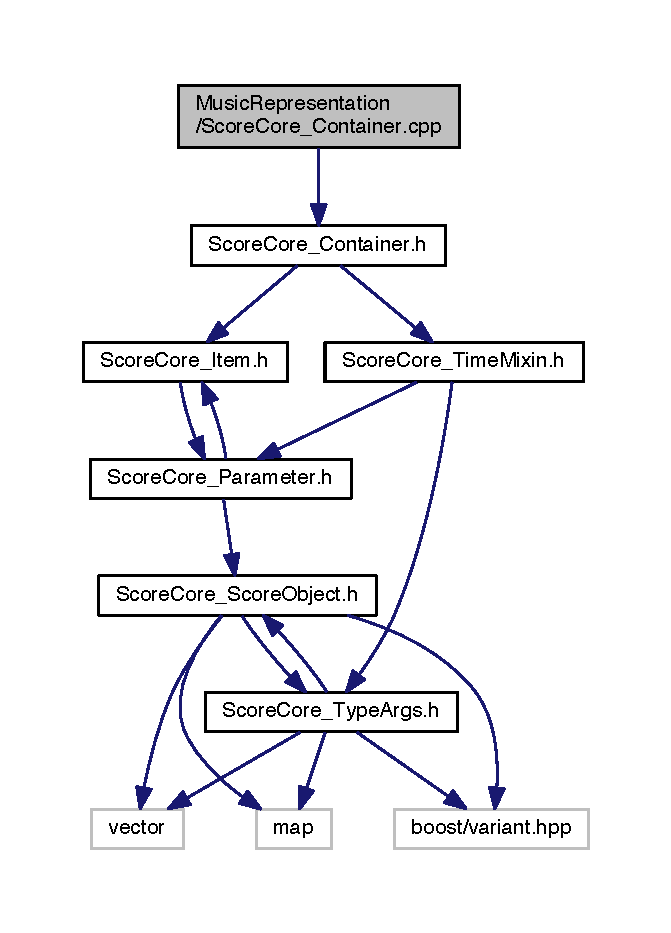
\includegraphics[width=322pt]{_score_core___container_8cpp__incl}
\end{center}
\end{figure}

\hypertarget{_score_core___container_8h}{\section{Music\-Representation/\-Score\-Core\-\_\-\-Container.h File Reference}
\label{_score_core___container_8h}\index{Music\-Representation/\-Score\-Core\-\_\-\-Container.\-h@{Music\-Representation/\-Score\-Core\-\_\-\-Container.\-h}}
}
{\ttfamily \#include \char`\"{}Score\-Core\-\_\-\-Item.\-h\char`\"{}}\\*
{\ttfamily \#include \char`\"{}Score\-Core\-\_\-\-Time\-Mixin.\-h\char`\"{}}\\*
Include dependency graph for Score\-Core\-\_\-\-Container.\-h\-:\nopagebreak
\begin{figure}[H]
\begin{center}
\leavevmode
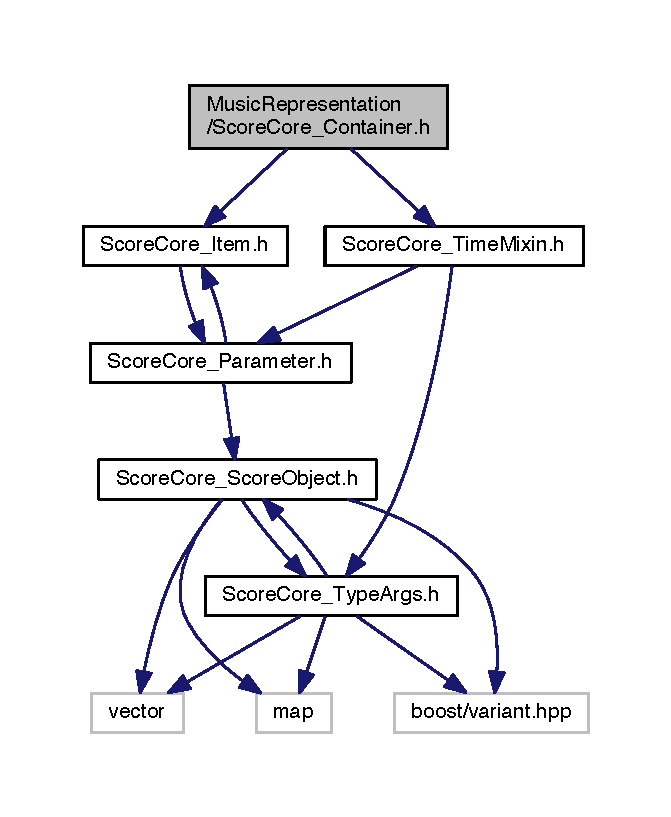
\includegraphics[width=322pt]{_score_core___container_8h__incl}
\end{center}
\end{figure}
This graph shows which files directly or indirectly include this file\-:\nopagebreak
\begin{figure}[H]
\begin{center}
\leavevmode
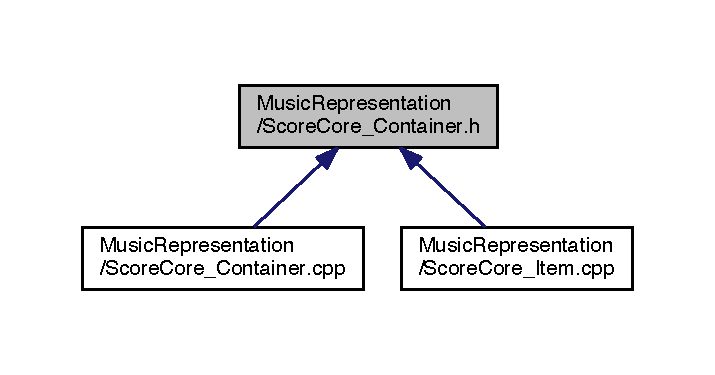
\includegraphics[width=343pt]{_score_core___container_8h__dep__incl}
\end{center}
\end{figure}
\subsection*{Classes}
\begin{DoxyCompactItemize}
\item 
class \hyperlink{class_container}{Container}
\item 
class \hyperlink{class_sequential}{Sequential}
\item 
class \hyperlink{class_simultaneous}{Simultaneous}
\end{DoxyCompactItemize}

\hypertarget{_score_core___element_8cpp}{\section{Music\-Representation/\-Score\-Core\-\_\-\-Element.cpp File Reference}
\label{_score_core___element_8cpp}\index{Music\-Representation/\-Score\-Core\-\_\-\-Element.\-cpp@{Music\-Representation/\-Score\-Core\-\_\-\-Element.\-cpp}}
}
{\ttfamily \#include \char`\"{}Score\-Core\-\_\-\-Element.\-h\char`\"{}}\\*
Include dependency graph for Score\-Core\-\_\-\-Element.\-cpp\-:\nopagebreak
\begin{figure}[H]
\begin{center}
\leavevmode
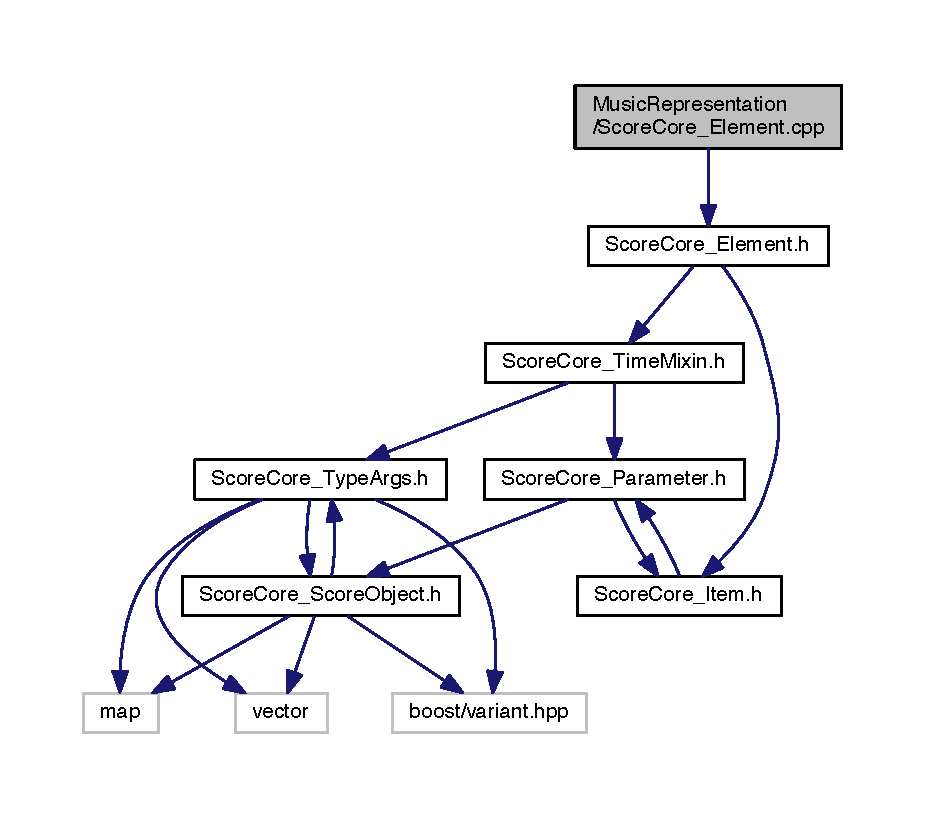
\includegraphics[width=350pt]{_score_core___element_8cpp__incl}
\end{center}
\end{figure}

\hypertarget{_score_core___element_8h}{\section{Music\-Representation/\-Score\-Core\-\_\-\-Element.h File Reference}
\label{_score_core___element_8h}\index{Music\-Representation/\-Score\-Core\-\_\-\-Element.\-h@{Music\-Representation/\-Score\-Core\-\_\-\-Element.\-h}}
}
{\ttfamily \#include \char`\"{}Score\-Core\-\_\-\-Time\-Mixin.\-h\char`\"{}}\\*
{\ttfamily \#include \char`\"{}Score\-Core\-\_\-\-Item.\-h\char`\"{}}\\*
Include dependency graph for Score\-Core\-\_\-\-Element.\-h\-:\nopagebreak
\begin{figure}[H]
\begin{center}
\leavevmode
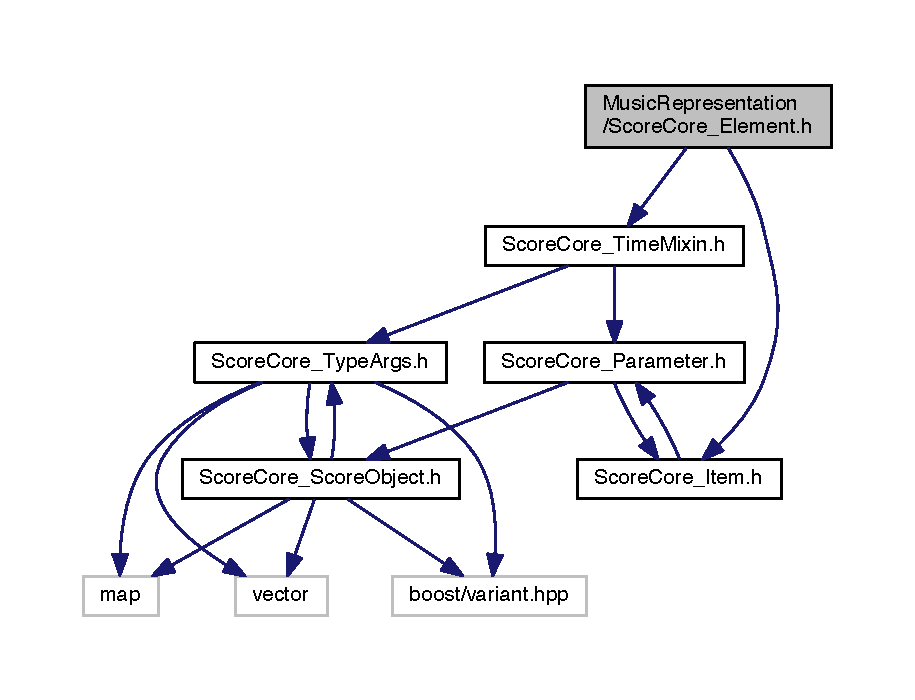
\includegraphics[width=350pt]{_score_core___element_8h__incl}
\end{center}
\end{figure}
This graph shows which files directly or indirectly include this file\-:\nopagebreak
\begin{figure}[H]
\begin{center}
\leavevmode
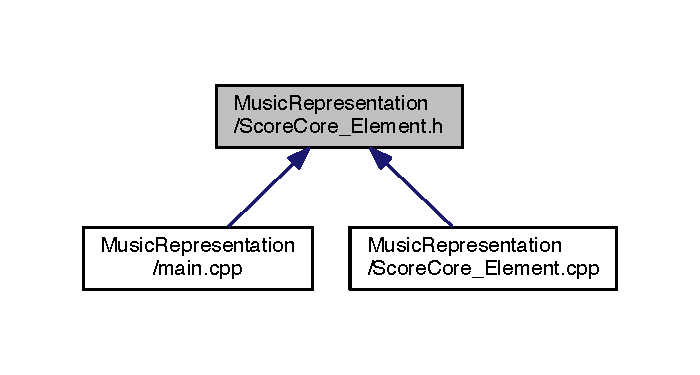
\includegraphics[width=336pt]{_score_core___element_8h__dep__incl}
\end{center}
\end{figure}
\subsection*{Classes}
\begin{DoxyCompactItemize}
\item 
class \hyperlink{class_element}{Element}
\end{DoxyCompactItemize}

\hypertarget{_score_core___item_8cpp}{\section{Music\-Representation/\-Score\-Core\-\_\-\-Item.cpp File Reference}
\label{_score_core___item_8cpp}\index{Music\-Representation/\-Score\-Core\-\_\-\-Item.\-cpp@{Music\-Representation/\-Score\-Core\-\_\-\-Item.\-cpp}}
}
{\ttfamily \#include \char`\"{}Score\-Core\-\_\-\-Item.\-h\char`\"{}}\\*
{\ttfamily \#include \char`\"{}Score\-Core\-\_\-\-Container.\-h\char`\"{}}\\*
Include dependency graph for Score\-Core\-\_\-\-Item.\-cpp\-:\nopagebreak
\begin{figure}[H]
\begin{center}
\leavevmode
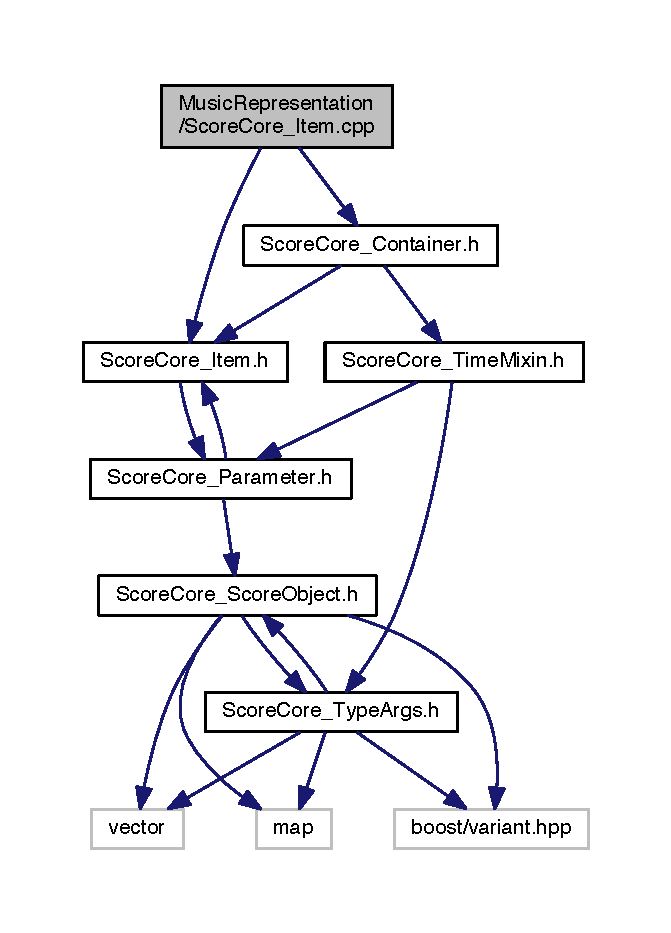
\includegraphics[width=322pt]{_score_core___item_8cpp__incl}
\end{center}
\end{figure}

\hypertarget{_score_core___item_8h}{\section{Music\-Representation/\-Score\-Core\-\_\-\-Item.h File Reference}
\label{_score_core___item_8h}\index{Music\-Representation/\-Score\-Core\-\_\-\-Item.\-h@{Music\-Representation/\-Score\-Core\-\_\-\-Item.\-h}}
}
{\ttfamily \#include \char`\"{}Score\-Core\-\_\-\-Parameter.\-h\char`\"{}}\\*
Include dependency graph for Score\-Core\-\_\-\-Item.\-h\-:\nopagebreak
\begin{figure}[H]
\begin{center}
\leavevmode
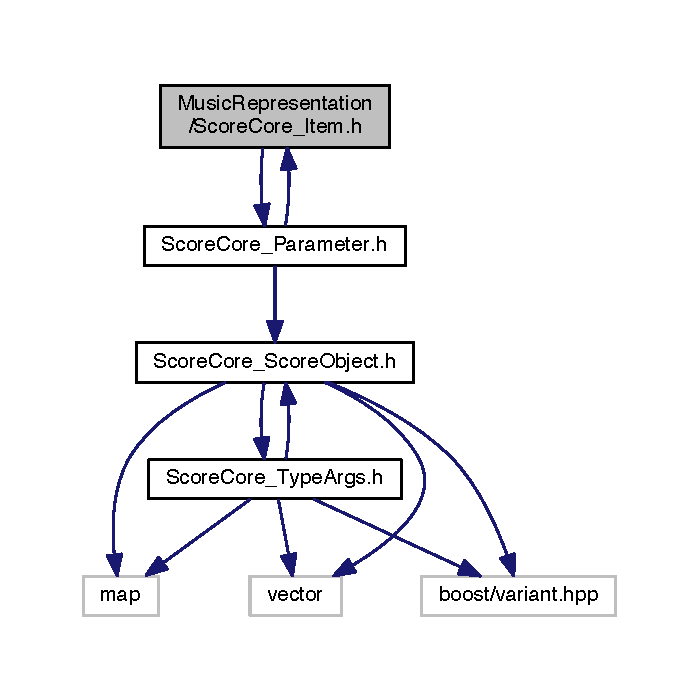
\includegraphics[width=335pt]{_score_core___item_8h__incl}
\end{center}
\end{figure}
This graph shows which files directly or indirectly include this file\-:\nopagebreak
\begin{figure}[H]
\begin{center}
\leavevmode
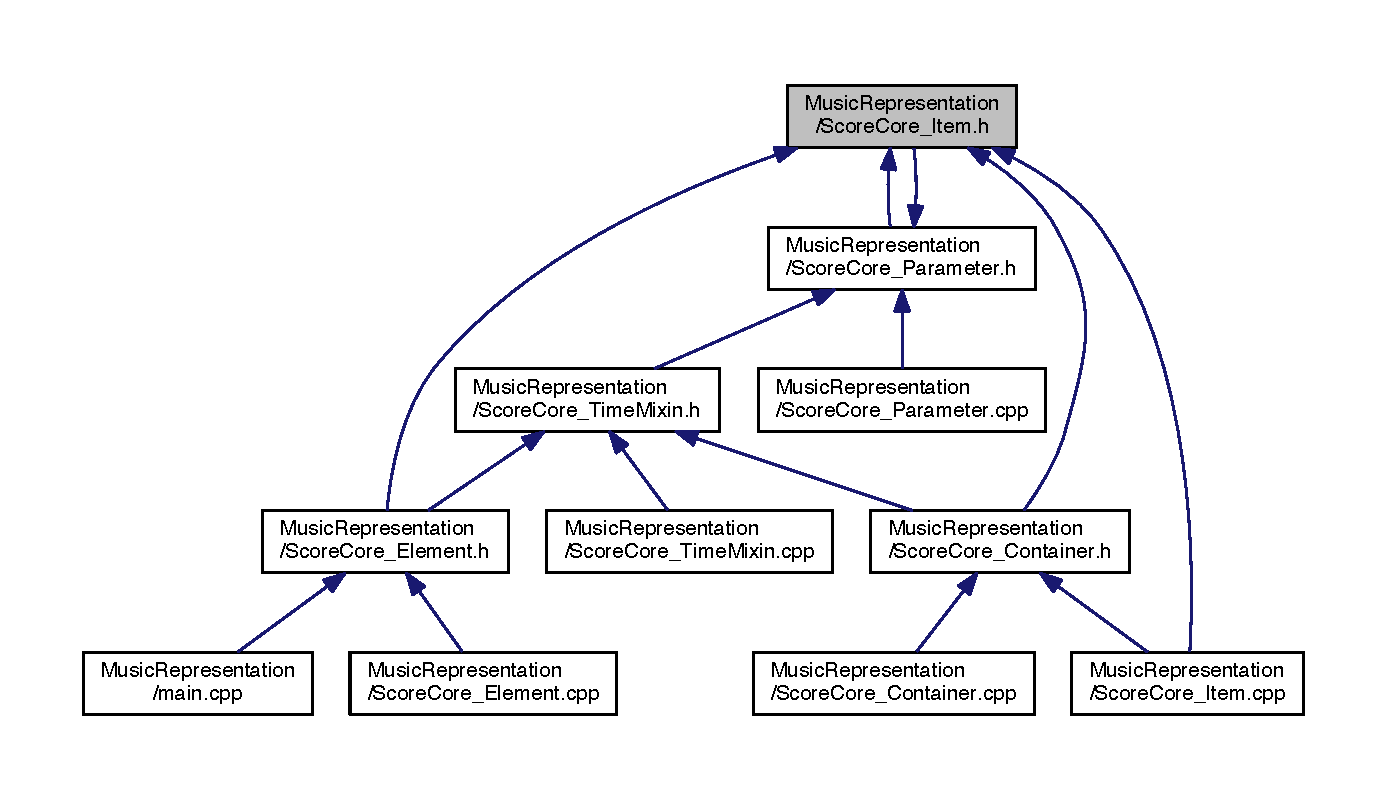
\includegraphics[width=350pt]{_score_core___item_8h__dep__incl}
\end{center}
\end{figure}
\subsection*{Classes}
\begin{DoxyCompactItemize}
\item 
class \hyperlink{class_item}{Item}
\end{DoxyCompactItemize}

\hypertarget{_score_core___parameter_8cpp}{\section{Music\-Representation/\-Score\-Core\-\_\-\-Parameter.cpp File Reference}
\label{_score_core___parameter_8cpp}\index{Music\-Representation/\-Score\-Core\-\_\-\-Parameter.\-cpp@{Music\-Representation/\-Score\-Core\-\_\-\-Parameter.\-cpp}}
}
{\ttfamily \#include \char`\"{}Score\-Core\-\_\-\-Parameter.\-h\char`\"{}}\\*
Include dependency graph for Score\-Core\-\_\-\-Parameter.\-cpp\-:\nopagebreak
\begin{figure}[H]
\begin{center}
\leavevmode
\includegraphics[width=350pt]{_score_core___parameter_8cpp__incl}
\end{center}
\end{figure}
\subsection*{Variables}
\begin{DoxyCompactItemize}
\item 
\hyperlink{_score_core___parameter_8cpp_afcc7a4b78ecd8fa7e713f8cfa0f51017}{value} \{\hyperlink{_score_core___type_args_8h_a935c216d448f8666d9675ab0a57f0afb}{extract\-Int\-Arg}(as, \char`\"{}value\char`\"{}, 0)\}
\item 
\hyperlink{_score_core___parameter_8cpp_a382b9040d9c3849b9350104bb5b3acfc}{unit}
\end{DoxyCompactItemize}


\subsection{Variable Documentation}
\hypertarget{_score_core___parameter_8cpp_a382b9040d9c3849b9350104bb5b3acfc}{\index{Score\-Core\-\_\-\-Parameter.\-cpp@{Score\-Core\-\_\-\-Parameter.\-cpp}!unit@{unit}}
\index{unit@{unit}!ScoreCore_Parameter.cpp@{Score\-Core\-\_\-\-Parameter.\-cpp}}
\subsubsection[{unit}]{\setlength{\rightskip}{0pt plus 5cm}unit}}\label{_score_core___parameter_8cpp_a382b9040d9c3849b9350104bb5b3acfc}
{\bfseries Initial value\-:}
\begin{DoxyCode}
\{\hyperlink{_score_core___type_args_8cpp_a53e66e3e10d8f092ae61c57ac808a159}{extractStringArg}(as, \textcolor{stringliteral}{"unit"}, \textcolor{stringliteral}{""})\}
\{
    
\}

\textcolor{keywordtype}{int} \hyperlink{class_parameter_a4459b636c3993ba40664ce8a53dad2c1}{Parameter::getValue}(\textcolor{keywordtype}{void}) \{ \textcolor{keywordflow}{return} value; \}
\textcolor{keywordtype}{string} \hyperlink{class_parameter_a0688af42890903c327ccf0b2373bff34}{Parameter::getUnit}(\textcolor{keywordtype}{void}) \{ \textcolor{keywordflow}{return} unit; \}
\hyperlink{class_item}{Item}* \hyperlink{class_parameter_ac2009f29ab47b8b68ae8739b348ec2c2}{Parameter::getItem}(\textcolor{keywordtype}{void}) \{ \textcolor{keywordflow}{return} item; \}
\end{DoxyCode}
\hypertarget{_score_core___parameter_8cpp_afcc7a4b78ecd8fa7e713f8cfa0f51017}{\index{Score\-Core\-\_\-\-Parameter.\-cpp@{Score\-Core\-\_\-\-Parameter.\-cpp}!value@{value}}
\index{value@{value}!ScoreCore_Parameter.cpp@{Score\-Core\-\_\-\-Parameter.\-cpp}}
\subsubsection[{value}]{\setlength{\rightskip}{0pt plus 5cm}value \{{\bf extract\-Int\-Arg}(as, \char`\"{}value\char`\"{}, 0)\}}}\label{_score_core___parameter_8cpp_afcc7a4b78ecd8fa7e713f8cfa0f51017}

\hypertarget{_score_core___parameter_8h}{\section{Music\-Representation/\-Score\-Core\-\_\-\-Parameter.h File Reference}
\label{_score_core___parameter_8h}\index{Music\-Representation/\-Score\-Core\-\_\-\-Parameter.\-h@{Music\-Representation/\-Score\-Core\-\_\-\-Parameter.\-h}}
}
{\ttfamily \#include \char`\"{}Score\-Core\-\_\-\-Score\-Object.\-h\char`\"{}}\\*
{\ttfamily \#include \char`\"{}Score\-Core\-\_\-\-Item.\-h\char`\"{}}\\*
Include dependency graph for Score\-Core\-\_\-\-Parameter.\-h\-:\nopagebreak
\begin{figure}[H]
\begin{center}
\leavevmode
\includegraphics[width=350pt]{_score_core___parameter_8h__incl}
\end{center}
\end{figure}
This graph shows which files directly or indirectly include this file\-:\nopagebreak
\begin{figure}[H]
\begin{center}
\leavevmode
\includegraphics[width=350pt]{_score_core___parameter_8h__dep__incl}
\end{center}
\end{figure}
\subsection*{Classes}
\begin{DoxyCompactItemize}
\item 
class \hyperlink{class_parameter}{Parameter}
\item 
class \hyperlink{class_time_parameter}{Time\-Parameter}
\item 
class \hyperlink{class_time_point}{Time\-Point}
\item 
class \hyperlink{class_time_interval}{Time\-Interval}
\item 
class \hyperlink{class_pitch}{Pitch}
\item 
class \hyperlink{class_amplitude}{Amplitude}
\end{DoxyCompactItemize}

\hypertarget{_score_core___score_object_8cpp}{\section{Music\-Representation/\-Score\-Core\-\_\-\-Score\-Object.cpp File Reference}
\label{_score_core___score_object_8cpp}\index{Music\-Representation/\-Score\-Core\-\_\-\-Score\-Object.\-cpp@{Music\-Representation/\-Score\-Core\-\_\-\-Score\-Object.\-cpp}}
}
{\ttfamily \#include \char`\"{}Score\-Core\-\_\-\-Score\-Object.\-h\char`\"{}}\\*
Include dependency graph for Score\-Core\-\_\-\-Score\-Object.\-cpp\-:\nopagebreak
\begin{figure}[H]
\begin{center}
\leavevmode
\includegraphics[width=335pt]{_score_core___score_object_8cpp__incl}
\end{center}
\end{figure}

\hypertarget{_score_core___score_object_8h}{\section{Music\-Representation/\-Score\-Core\-\_\-\-Score\-Object.h File Reference}
\label{_score_core___score_object_8h}\index{Music\-Representation/\-Score\-Core\-\_\-\-Score\-Object.\-h@{Music\-Representation/\-Score\-Core\-\_\-\-Score\-Object.\-h}}
}
{\ttfamily \#include $<$map$>$}\\*
{\ttfamily \#include $<$vector$>$}\\*
{\ttfamily \#include $<$boost/variant.\-hpp$>$}\\*
{\ttfamily \#include \char`\"{}Score\-Core\-\_\-\-Type\-Args.\-h\char`\"{}}\\*
Include dependency graph for Score\-Core\-\_\-\-Score\-Object.\-h\-:\nopagebreak
\begin{figure}[H]
\begin{center}
\leavevmode
\includegraphics[width=335pt]{_score_core___score_object_8h__incl}
\end{center}
\end{figure}
This graph shows which files directly or indirectly include this file\-:\nopagebreak
\begin{figure}[H]
\begin{center}
\leavevmode
\includegraphics[width=350pt]{_score_core___score_object_8h__dep__incl}
\end{center}
\end{figure}
\subsection*{Classes}
\begin{DoxyCompactItemize}
\item 
class \hyperlink{class_score_object}{Score\-Object}
\end{DoxyCompactItemize}
\subsection*{Typedefs}
\begin{DoxyCompactItemize}
\item 
typedef std\-::map$<$ std\-::string, \\*
boost\-::variant$<$ int, \\*
std\-::string, \hyperlink{class_score_object}{Score\-Object}, \\*
std\-::vector$<$ \hyperlink{class_score_object}{Score\-Object} $>$ $>$ $>$ \hyperlink{_score_core___score_object_8h_ab88aad89d974920ebfb0b0c9e46f61b4}{Args}
\end{DoxyCompactItemize}


\subsection{Typedef Documentation}
\hypertarget{_score_core___score_object_8h_ab88aad89d974920ebfb0b0c9e46f61b4}{\index{Score\-Core\-\_\-\-Score\-Object.\-h@{Score\-Core\-\_\-\-Score\-Object.\-h}!Args@{Args}}
\index{Args@{Args}!ScoreCore_ScoreObject.h@{Score\-Core\-\_\-\-Score\-Object.\-h}}
\subsubsection[{Args}]{\setlength{\rightskip}{0pt plus 5cm}typedef std\-::map$<$std\-::string, boost\-::variant$<$int,std\-::string,{\bf Score\-Object},std\-::vector$<${\bf Score\-Object}$>$ $>$ $>$ {\bf Args}}}\label{_score_core___score_object_8h_ab88aad89d974920ebfb0b0c9e46f61b4}

\hypertarget{_score_core___time_mixin_8cpp}{\section{Music\-Representation/\-Score\-Core\-\_\-\-Time\-Mixin.cpp File Reference}
\label{_score_core___time_mixin_8cpp}\index{Music\-Representation/\-Score\-Core\-\_\-\-Time\-Mixin.\-cpp@{Music\-Representation/\-Score\-Core\-\_\-\-Time\-Mixin.\-cpp}}
}
{\ttfamily \#include \char`\"{}Score\-Core\-\_\-\-Time\-Mixin.\-h\char`\"{}}\\*
Include dependency graph for Score\-Core\-\_\-\-Time\-Mixin.\-cpp\-:\nopagebreak
\begin{figure}[H]
\begin{center}
\leavevmode
\includegraphics[width=350pt]{_score_core___time_mixin_8cpp__incl}
\end{center}
\end{figure}

\hypertarget{_score_core___time_mixin_8h}{\section{Music\-Representation/\-Score\-Core\-\_\-\-Time\-Mixin.h File Reference}
\label{_score_core___time_mixin_8h}\index{Music\-Representation/\-Score\-Core\-\_\-\-Time\-Mixin.\-h@{Music\-Representation/\-Score\-Core\-\_\-\-Time\-Mixin.\-h}}
}
{\ttfamily \#include \char`\"{}Score\-Core\-\_\-\-Type\-Args.\-h\char`\"{}}\\*
{\ttfamily \#include \char`\"{}Score\-Core\-\_\-\-Parameter.\-h\char`\"{}}\\*
Include dependency graph for Score\-Core\-\_\-\-Time\-Mixin.\-h\-:\nopagebreak
\begin{figure}[H]
\begin{center}
\leavevmode
\includegraphics[width=350pt]{_score_core___time_mixin_8h__incl}
\end{center}
\end{figure}
This graph shows which files directly or indirectly include this file\-:\nopagebreak
\begin{figure}[H]
\begin{center}
\leavevmode
\includegraphics[width=350pt]{_score_core___time_mixin_8h__dep__incl}
\end{center}
\end{figure}
\subsection*{Classes}
\begin{DoxyCompactItemize}
\item 
class \hyperlink{class_time_mixin}{Time\-Mixin}
\end{DoxyCompactItemize}

\hypertarget{_score_core___type_args_8cpp}{\section{Music\-Representation/\-Score\-Core\-\_\-\-Type\-Args.cpp File Reference}
\label{_score_core___type_args_8cpp}\index{Music\-Representation/\-Score\-Core\-\_\-\-Type\-Args.\-cpp@{Music\-Representation/\-Score\-Core\-\_\-\-Type\-Args.\-cpp}}
}
{\ttfamily \#include $<$boost/lexical\-\_\-cast.\-hpp$>$}\\*
{\ttfamily \#include \char`\"{}Score\-Core\-\_\-\-Type\-Args.\-h\char`\"{}}\\*
Include dependency graph for Score\-Core\-\_\-\-Type\-Args.\-cpp\-:\nopagebreak
\begin{figure}[H]
\begin{center}
\leavevmode
\includegraphics[width=350pt]{_score_core___type_args_8cpp__incl}
\end{center}
\end{figure}
\subsection*{Functions}
\begin{DoxyCompactItemize}
\item 
\hyperlink{_score_core___score_object_8h_ab88aad89d974920ebfb0b0c9e46f61b4}{Args} \hyperlink{_score_core___type_args_8cpp_ab92694a264be4616c96b5d209758c76a}{reduce\-Args\-By} (\hyperlink{_score_core___score_object_8h_ab88aad89d974920ebfb0b0c9e46f61b4}{Args} as, vector$<$ string $>$ keys)
\item 
int \hyperlink{_score_core___type_args_8cpp_af74d14e18f1057351d30da7a99327d8a}{extract\-Int\-Arg} (\hyperlink{_score_core___score_object_8h_ab88aad89d974920ebfb0b0c9e46f61b4}{Args} as, string arg\-Name, int default\-Val)
\item 
string \hyperlink{_score_core___type_args_8cpp_a53e66e3e10d8f092ae61c57ac808a159}{extract\-String\-Arg} (\hyperlink{_score_core___score_object_8h_ab88aad89d974920ebfb0b0c9e46f61b4}{Args} as, string arg\-Name, string default\-Val)
\item 
std\-::vector$<$ \hyperlink{class_score_object}{Score\-Object} $>$ \hyperlink{_score_core___type_args_8cpp_ae5303d031357dddab2b55a2f391e2685}{extract\-Vector\-Of\-Score\-Objects\-Arg} (\hyperlink{_score_core___score_object_8h_ab88aad89d974920ebfb0b0c9e46f61b4}{Args} as, string arg\-Name)
\end{DoxyCompactItemize}


\subsection{Detailed Description}
Defines types and classes which allow to quasi hand optional and named parameters to score object constructors. These parameters are wrapped in a map called Args. 

\subsection{Function Documentation}
\hypertarget{_score_core___type_args_8cpp_af74d14e18f1057351d30da7a99327d8a}{\index{Score\-Core\-\_\-\-Type\-Args.\-cpp@{Score\-Core\-\_\-\-Type\-Args.\-cpp}!extract\-Int\-Arg@{extract\-Int\-Arg}}
\index{extract\-Int\-Arg@{extract\-Int\-Arg}!ScoreCore_TypeArgs.cpp@{Score\-Core\-\_\-\-Type\-Args.\-cpp}}
\subsubsection[{extract\-Int\-Arg}]{\setlength{\rightskip}{0pt plus 5cm}int extract\-Int\-Arg (
\begin{DoxyParamCaption}
\item[{{\bf Args}}]{as, }
\item[{string}]{arg\-Name, }
\item[{int}]{default\-Val}
\end{DoxyParamCaption}
)}}\label{_score_core___type_args_8cpp_af74d14e18f1057351d30da7a99327d8a}
Extracts arg named arg\-Name from Args map as. If not contained in as, then default\-Val is return instead. \hypertarget{_score_core___type_args_8cpp_a53e66e3e10d8f092ae61c57ac808a159}{\index{Score\-Core\-\_\-\-Type\-Args.\-cpp@{Score\-Core\-\_\-\-Type\-Args.\-cpp}!extract\-String\-Arg@{extract\-String\-Arg}}
\index{extract\-String\-Arg@{extract\-String\-Arg}!ScoreCore_TypeArgs.cpp@{Score\-Core\-\_\-\-Type\-Args.\-cpp}}
\subsubsection[{extract\-String\-Arg}]{\setlength{\rightskip}{0pt plus 5cm}string extract\-String\-Arg (
\begin{DoxyParamCaption}
\item[{{\bf Args}}]{as, }
\item[{string}]{arg\-Name, }
\item[{string}]{default\-Val}
\end{DoxyParamCaption}
)}}\label{_score_core___type_args_8cpp_a53e66e3e10d8f092ae61c57ac808a159}
\hypertarget{_score_core___type_args_8cpp_ae5303d031357dddab2b55a2f391e2685}{\index{Score\-Core\-\_\-\-Type\-Args.\-cpp@{Score\-Core\-\_\-\-Type\-Args.\-cpp}!extract\-Vector\-Of\-Score\-Objects\-Arg@{extract\-Vector\-Of\-Score\-Objects\-Arg}}
\index{extract\-Vector\-Of\-Score\-Objects\-Arg@{extract\-Vector\-Of\-Score\-Objects\-Arg}!ScoreCore_TypeArgs.cpp@{Score\-Core\-\_\-\-Type\-Args.\-cpp}}
\subsubsection[{extract\-Vector\-Of\-Score\-Objects\-Arg}]{\setlength{\rightskip}{0pt plus 5cm}std\-::vector$<${\bf Score\-Object}$>$ extract\-Vector\-Of\-Score\-Objects\-Arg (
\begin{DoxyParamCaption}
\item[{{\bf Args}}]{as, }
\item[{string}]{arg\-Name}
\end{DoxyParamCaption}
)}}\label{_score_core___type_args_8cpp_ae5303d031357dddab2b55a2f391e2685}
\hypertarget{_score_core___type_args_8cpp_ab92694a264be4616c96b5d209758c76a}{\index{Score\-Core\-\_\-\-Type\-Args.\-cpp@{Score\-Core\-\_\-\-Type\-Args.\-cpp}!reduce\-Args\-By@{reduce\-Args\-By}}
\index{reduce\-Args\-By@{reduce\-Args\-By}!ScoreCore_TypeArgs.cpp@{Score\-Core\-\_\-\-Type\-Args.\-cpp}}
\subsubsection[{reduce\-Args\-By}]{\setlength{\rightskip}{0pt plus 5cm}{\bf Args} reduce\-Args\-By (
\begin{DoxyParamCaption}
\item[{{\bf Args}}]{as, }
\item[{vector$<$ string $>$}]{keys}
\end{DoxyParamCaption}
)}}\label{_score_core___type_args_8cpp_ab92694a264be4616c96b5d209758c76a}
Returns a copy of Args map as, reduced by the keys in keys 
\hypertarget{_score_core___type_args_8h}{\section{Music\-Representation/\-Score\-Core\-\_\-\-Type\-Args.h File Reference}
\label{_score_core___type_args_8h}\index{Music\-Representation/\-Score\-Core\-\_\-\-Type\-Args.\-h@{Music\-Representation/\-Score\-Core\-\_\-\-Type\-Args.\-h}}
}
{\ttfamily \#include $<$map$>$}\\*
{\ttfamily \#include $<$vector$>$}\\*
{\ttfamily \#include $<$boost/variant.\-hpp$>$}\\*
{\ttfamily \#include \char`\"{}Score\-Core\-\_\-\-Score\-Object.\-h\char`\"{}}\\*
Include dependency graph for Score\-Core\-\_\-\-Type\-Args.\-h\-:\nopagebreak
\begin{figure}[H]
\begin{center}
\leavevmode
\includegraphics[width=342pt]{_score_core___type_args_8h__incl}
\end{center}
\end{figure}
This graph shows which files directly or indirectly include this file\-:\nopagebreak
\begin{figure}[H]
\begin{center}
\leavevmode
\includegraphics[width=350pt]{_score_core___type_args_8h__dep__incl}
\end{center}
\end{figure}
\subsection*{Classes}
\begin{DoxyCompactItemize}
\item 
class \hyperlink{classget_string_arg}{get\-String\-Arg}
\item 
class \hyperlink{classget_int_arg}{get\-Int\-Arg}
\item 
class \hyperlink{classget_score_object_arg}{get\-Score\-Object\-Arg}
\item 
class \hyperlink{classget_vector_of_score_objects_arg}{get\-Vector\-Of\-Score\-Objects\-Arg}
\item 
class \hyperlink{classget_arg}{get\-Arg$<$ T $>$}
\end{DoxyCompactItemize}
\subsection*{Typedefs}
\begin{DoxyCompactItemize}
\item 
typedef std\-::map$<$ std\-::string, \\*
boost\-::variant$<$ int, \\*
std\-::string, \hyperlink{class_score_object}{Score\-Object}, \\*
std\-::vector$<$ \hyperlink{class_score_object}{Score\-Object} $>$ $>$ $>$ \hyperlink{_score_core___type_args_8h_ab88aad89d974920ebfb0b0c9e46f61b4}{Args}
\end{DoxyCompactItemize}
\subsection*{Functions}
\begin{DoxyCompactItemize}
\item 
\hyperlink{_score_core___score_object_8h_ab88aad89d974920ebfb0b0c9e46f61b4}{Args} \hyperlink{_score_core___type_args_8h_a91b0ccfcc279cb0c6f2ba3b5a7c168b6}{reduce\-Args\-By} (\hyperlink{_score_core___score_object_8h_ab88aad89d974920ebfb0b0c9e46f61b4}{Args} as, std\-::vector$<$ std\-::string $>$ keys)
\item 
int \hyperlink{_score_core___type_args_8h_a935c216d448f8666d9675ab0a57f0afb}{extract\-Int\-Arg} (\hyperlink{_score_core___score_object_8h_ab88aad89d974920ebfb0b0c9e46f61b4}{Args} as, std\-::string arg\-Name, int default\-Val)
\item 
std\-::string \hyperlink{_score_core___type_args_8h_ad43ee7ead79eb9393c5ad9e3656dcc88}{extract\-String\-Arg} (\hyperlink{_score_core___score_object_8h_ab88aad89d974920ebfb0b0c9e46f61b4}{Args} as, std\-::string arg\-Name, std\-::string default\-Val)
\item 
std\-::vector$<$ \hyperlink{class_score_object}{Score\-Object} $>$ \hyperlink{_score_core___type_args_8h_a85a0948e38d5c074c4ff102a47632468}{extract\-Vector\-Of\-Score\-Objects\-Arg} (\hyperlink{_score_core___score_object_8h_ab88aad89d974920ebfb0b0c9e46f61b4}{Args} as, std\-::string arg\-Name)
\end{DoxyCompactItemize}


\subsection{Detailed Description}
Defines types and classes which allow to quasi hand optional and named parameters to score object constructors. These parameters are wrapped in a map called Args. 

\subsection{Typedef Documentation}
\hypertarget{_score_core___type_args_8h_ab88aad89d974920ebfb0b0c9e46f61b4}{\index{Score\-Core\-\_\-\-Type\-Args.\-h@{Score\-Core\-\_\-\-Type\-Args.\-h}!Args@{Args}}
\index{Args@{Args}!ScoreCore_TypeArgs.h@{Score\-Core\-\_\-\-Type\-Args.\-h}}
\subsubsection[{Args}]{\setlength{\rightskip}{0pt plus 5cm}typedef std\-::map$<$std\-::string, boost\-::variant$<$int,std\-::string,{\bf Score\-Object},std\-::vector$<${\bf Score\-Object}$>$ $>$ $>$ {\bf Args}}}\label{_score_core___type_args_8h_ab88aad89d974920ebfb0b0c9e46f61b4}
Shorthand type for argument maps for score object constructors. This type effectively allows for optional and named arguments for constructors of \hyperlink{class_score_object}{Score\-Object} and subclasses. You can conveniently create such named arguments like

Some\-Score\-Object\-Class x = \{Args \{\{\char`\"{}arg1\char`\"{}, 42\}, \{\char`\"{}arg2\char`\"{}, \char`\"{}test\char`\"{}\}\}\}

\begin{DoxySeeAlso}{See Also}
The constructors of \hyperlink{class_score_object}{Score\-Object} and its subclasses. 
\end{DoxySeeAlso}


\subsection{Function Documentation}
\hypertarget{_score_core___type_args_8h_a935c216d448f8666d9675ab0a57f0afb}{\index{Score\-Core\-\_\-\-Type\-Args.\-h@{Score\-Core\-\_\-\-Type\-Args.\-h}!extract\-Int\-Arg@{extract\-Int\-Arg}}
\index{extract\-Int\-Arg@{extract\-Int\-Arg}!ScoreCore_TypeArgs.h@{Score\-Core\-\_\-\-Type\-Args.\-h}}
\subsubsection[{extract\-Int\-Arg}]{\setlength{\rightskip}{0pt plus 5cm}int extract\-Int\-Arg (
\begin{DoxyParamCaption}
\item[{{\bf Args}}]{as, }
\item[{std\-::string}]{arg\-Name, }
\item[{int}]{default\-Val}
\end{DoxyParamCaption}
)}}\label{_score_core___type_args_8h_a935c216d448f8666d9675ab0a57f0afb}
Extracts arg named arg\-Name from Args map as. If not contained in as, then default\-Val is return instead. \hypertarget{_score_core___type_args_8h_ad43ee7ead79eb9393c5ad9e3656dcc88}{\index{Score\-Core\-\_\-\-Type\-Args.\-h@{Score\-Core\-\_\-\-Type\-Args.\-h}!extract\-String\-Arg@{extract\-String\-Arg}}
\index{extract\-String\-Arg@{extract\-String\-Arg}!ScoreCore_TypeArgs.h@{Score\-Core\-\_\-\-Type\-Args.\-h}}
\subsubsection[{extract\-String\-Arg}]{\setlength{\rightskip}{0pt plus 5cm}std\-::string extract\-String\-Arg (
\begin{DoxyParamCaption}
\item[{{\bf Args}}]{as, }
\item[{std\-::string}]{arg\-Name, }
\item[{std\-::string}]{default\-Val}
\end{DoxyParamCaption}
)}}\label{_score_core___type_args_8h_ad43ee7ead79eb9393c5ad9e3656dcc88}
\hypertarget{_score_core___type_args_8h_a85a0948e38d5c074c4ff102a47632468}{\index{Score\-Core\-\_\-\-Type\-Args.\-h@{Score\-Core\-\_\-\-Type\-Args.\-h}!extract\-Vector\-Of\-Score\-Objects\-Arg@{extract\-Vector\-Of\-Score\-Objects\-Arg}}
\index{extract\-Vector\-Of\-Score\-Objects\-Arg@{extract\-Vector\-Of\-Score\-Objects\-Arg}!ScoreCore_TypeArgs.h@{Score\-Core\-\_\-\-Type\-Args.\-h}}
\subsubsection[{extract\-Vector\-Of\-Score\-Objects\-Arg}]{\setlength{\rightskip}{0pt plus 5cm}std\-::vector$<${\bf Score\-Object}$>$ extract\-Vector\-Of\-Score\-Objects\-Arg (
\begin{DoxyParamCaption}
\item[{{\bf Args}}]{as, }
\item[{std\-::string}]{arg\-Name}
\end{DoxyParamCaption}
)}}\label{_score_core___type_args_8h_a85a0948e38d5c074c4ff102a47632468}
\hypertarget{_score_core___type_args_8h_a91b0ccfcc279cb0c6f2ba3b5a7c168b6}{\index{Score\-Core\-\_\-\-Type\-Args.\-h@{Score\-Core\-\_\-\-Type\-Args.\-h}!reduce\-Args\-By@{reduce\-Args\-By}}
\index{reduce\-Args\-By@{reduce\-Args\-By}!ScoreCore_TypeArgs.h@{Score\-Core\-\_\-\-Type\-Args.\-h}}
\subsubsection[{reduce\-Args\-By}]{\setlength{\rightskip}{0pt plus 5cm}{\bf Args} reduce\-Args\-By (
\begin{DoxyParamCaption}
\item[{{\bf Args}}]{as, }
\item[{std\-::vector$<$ std\-::string $>$}]{keys}
\end{DoxyParamCaption}
)}}\label{_score_core___type_args_8h_a91b0ccfcc279cb0c6f2ba3b5a7c168b6}
Returns a copy of Args map as, reduced by the keys in keys 
\hypertarget{_score_mapping_8cpp}{\section{Music\-Representation/\-Score\-Mapping.cpp File Reference}
\label{_score_mapping_8cpp}\index{Music\-Representation/\-Score\-Mapping.\-cpp@{Music\-Representation/\-Score\-Mapping.\-cpp}}
}
{\ttfamily \#include $<$vector$>$}\\*
{\ttfamily \#include \char`\"{}Score\-Mapping.\-h\char`\"{}}\\*
Include dependency graph for Score\-Mapping.\-cpp\-:\nopagebreak
\begin{figure}[H]
\begin{center}
\leavevmode
\includegraphics[width=231pt]{_score_mapping_8cpp__incl}
\end{center}
\end{figure}
\subsection*{Namespaces}
\begin{DoxyCompactItemize}
\item 
\hyperlink{namespace_strasheela_successor}{Strasheela\-Successor}
\end{DoxyCompactItemize}

\hypertarget{_score_mapping_8h}{\section{Music\-Representation/\-Score\-Mapping.h File Reference}
\label{_score_mapping_8h}\index{Music\-Representation/\-Score\-Mapping.\-h@{Music\-Representation/\-Score\-Mapping.\-h}}
}
This graph shows which files directly or indirectly include this file\-:\nopagebreak
\begin{figure}[H]
\begin{center}
\leavevmode
\includegraphics[width=190pt]{_score_mapping_8h__dep__incl}
\end{center}
\end{figure}
\subsection*{Namespaces}
\begin{DoxyCompactItemize}
\item 
\hyperlink{namespace_strasheela_successor}{Strasheela\-Successor}
\end{DoxyCompactItemize}

%--- End generated contents ---

% Index
\newpage
\phantomsection
\addcontentsline{toc}{chapter}{Index}
\printindex

\end{document}
